%!TEX root = these.tex

\chapter[Visual Analytics et approches sémantiques pour la biologie moléculaire]{Visual Analytics et approches sémantiques pour la biologie moléculaire}
\label{Sec:VisuAna_def}
\minitoc
\cleardoublepage

%Nos efforts pour décrire la boucle de travail des experts en biologie structurale ne peuvent se restreindre aux étapes de génération des données représentées par les étapes (1) et (2) de la Figure \ref{Fig:schema_seq_bio_struct}. 


Les tâches conjointes d'analyse et de visualisation des données générées par simulation moléculaire ont pour objectifs, d'une part de confirmer la cohérence et la validité d'un résultat théoriques de simulation au regard de des résultats expérimentaux scientifiques établis, et d'autre part d'aider l'expert à formuler de nouvelles hypothèses à confirmer ensuite de manière expérimentale. Nous avons vu qu'au sein du processus d'étude de structures moléculaires, ces deux espaces de travail mobilisant des outils variés sont omniprésents dans chacune des étapes du processus, depuis l'expérimentation, jusqu'à la simulation en passant par la modélisation et la visualisation. Nous rappelons que les objectifs de ce travail est de minimiser les données échangées entre les étapes de visualisation et d'analyse, en rapprochant les étapes de simulation, de visualisation, d'analyse tout en permettant à l'expert de pouvoir effectuer des visualisations et des analyses à la demande sur le lieu de simulation. il s'agit aussi de répondre aux contraintes propres aux environnement immersifs pour les rendre opérationnels pour le domaine de la biologie moléculaire, en favorisant les interactions directes dans un  contexte interactif commun. Pour répondre à ces objectifs, nous avons emprunté des concepts issus des approches de type Visual Analytics, mobilisant des concepts de représentation sémantique des connaissances. Nous présentons donc dans ce chapitre un aperçu des concepts et des techniques relatives à ces deux domaines, de leurs applications aux domaines de la biologie, pré-requis nécessaire pour présenter notre contribution dans le dernier chapitre adressant les deux objectifs précités. 

%Pour permettre à l'expert une compréhension globale de son système, il est nécessaire d'intégrer les données analysées au sein d'un espace de visualisation capable d'explorer des complexes moléculaires de grande taille. La RV met en jeu un espace immersif dont les méthodes d'interactions demandent une interactivité des données mises en jeu. Cette interactivité mettant en jeu visualisation et données complexes est justement le concept clé dirigeant le domaine du \textit{\textbf{Visual Analytics}}.


%Même si plus discret, car plus large, le domaine du \textit{Big Data} et des analyses de données massives qui lui sont associées sont aujourd'hui au cœur de nombreux projets.

% Nous avons décrit les différentes facettes de la visualisation, moyen de compréhension, communication et création de nouvelles connaissances.
% Dans le cadre exposé en introduction d'une complexité toujours plus importante des modèles 3d de protéines, la navigation guidée par le contenu et la tâche présentée dans le chapitre précédent constitue une solution à l'exploration de ces complexes de grande taille au sein de cette de visualisation. Mais si elle offre la possibilité d'explorer de façon immersive des contenus moléculaires complexes, elle ne permet par contre pas de réduire leur complexité ou la complexité des propriétés associées. La problématique de la complexité des données manipulées et échangées entre les différentes étapes du processus reste donc intacte.

% Le traitement analytique de la simulation moléculaire peut amener l'utilisateur à . La simulation est la principale génératrice de nouvelles données brutes à interpréter et analyser et est donc en grande partie responsable de la surcharge de données du processus de biologie structurale. Cependant l'analyse joue également un rôle central dans la génération de connaissances, souvent sous forme de valeurs brutes venant complémenter et expliquer les données de la simulation.
% L'analyse constitue donc un autre goulot d'étranglement pour le flux de données.




%%%%%%%%%%%%%%%%%%%%% DEBUT INTRO FROM CHAP.2 %%%%%%%%%%%%%%%%%%%%%%%%%%%%%%%

\section{Visual Analytics : définition, outils et applications}

%Une première pierre pour cette réflexion pourrait venir, selon nous, du domaine de la visualisation analytique et de ses problématiques, parfois proches de celles que nous retrouvons en RV.
Lorsque l'on s'intéresse à la place des approches par Visual Analytics dans les disciplines de biologie et de médecine (voir Figure \ref{Fig:VA_pubmed_trend}), on s'aperçoit que ce domaine émergent connaît une progression identique à celle de la RV. Nous expliquons cette croissance par l'observation partagée de la communauté de trouver de nouvelles approches pour répondre à la problématique centrale relative à  la quantité de données à visualiser et à analyser.

\begin{figure}
  \centering
  {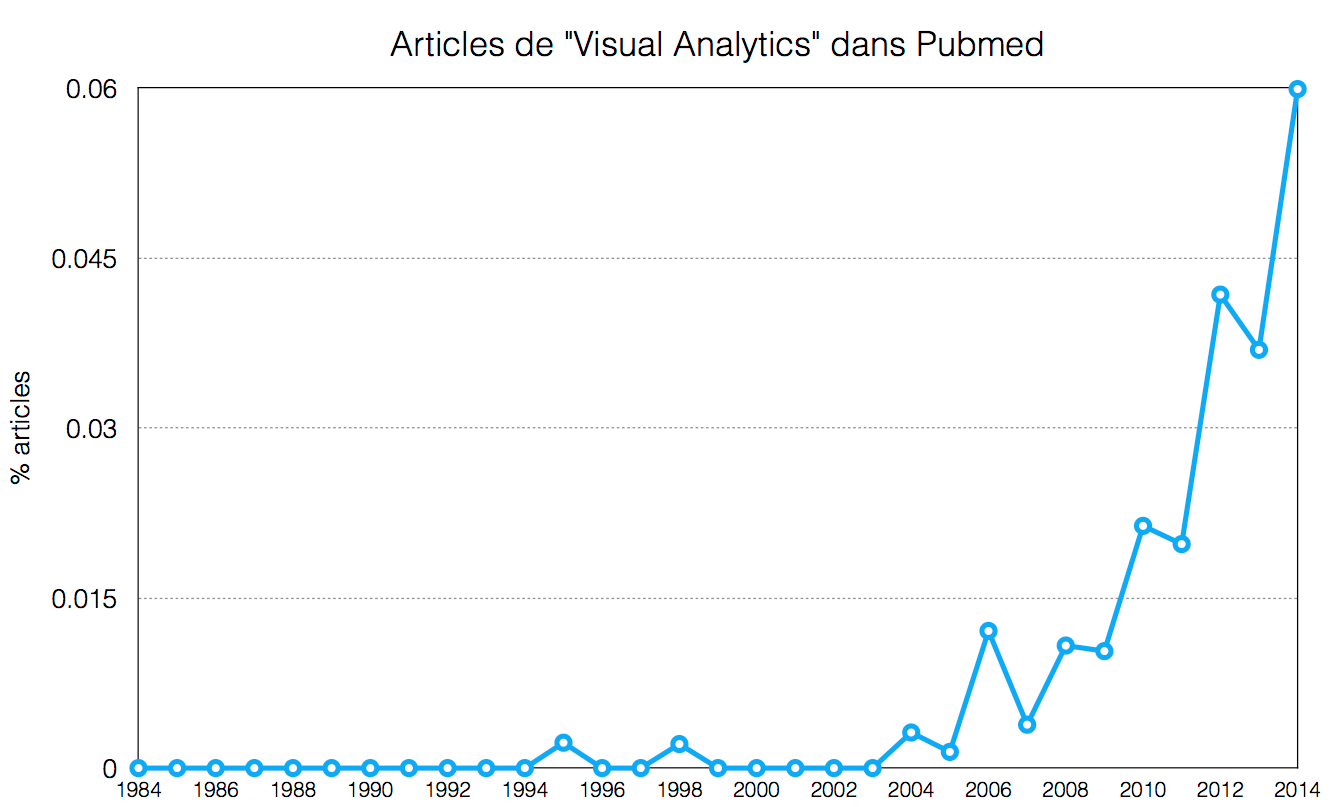
\includegraphics[width=.75\linewidth]{./figures/ch4/VA_pubmed_trend.png}}
    \caption[Évolution des articles traitant de \textit{Visual Analytics} dans PubMed.]{{\it Evolution du pourcentage d'articles de PubMed où le terme <<Visual Analytics>> est retrouvé soit dans le titre soit dans le résumé au cours des 20 dernières années.}}
  \label{Fig:VA_pubmed_trend}
  \hspace{0.3cm}
\end{figure}

L'association par des liens interactifs, de plusieurs représentations visuelles de données souvent hétérogènes,  dans un même espace de travail, nécessitent l'introduction de nouvelles techniques de visualisation définies dans le cadre d'un domaine de recherche émergent appelé \textit{Visual Analytics}.

\subsection{Définition}

Cette discipline récente a pour but de faciliter l'analyse visuelle de données complexes et/ou scientifiques et se définit par le <<raisonnement analytique au travers d'interfaces visuelles interactives>> \cite{cook_illuminating_2005}. Elle se place à la frontière de nombreux domaines, comme celui de la visualisation, de l'interaction homme-machine et de perception, afin de visuellement mettre en avant des relations entre les informations, difficiles à percevoir lors de l'utilisation cloisonnée de techniques classiques issues de ces différents domaines. %les approches par Visual Analytics s'appuient sur des méthodes de visualisation simples et compréhensibles par l'être humain auxquelles elle ajoute une dimension interactive afin de les relier entre elles. 
Elle s'inspire donc par plusieurs niveaux aux études d'interactions homme-machine (IHM) dont la réalité virtuelle s'inspire également \cite{arias-hernandez_visual_2011}. De la même manière qu'en IHM, elle se repose sur des outils et des techniques basées sur des considérations ergonomiques et perceptuelles. Son principal but est de mettre l'être humain au centre d'une boucle de décision qui sera facilitée par la mise en relation de données de différentes natures et de différentes sources. Ce contexte de travail généré par la visualisation analytique doit être cohérent pour le chercheur. C'est à ce niveau que les domaines de la perception et des études cognitives interviennent afin d'assurer une pleine compréhension et utilisation de l'espace de travail. La VA se place comme un catalyseur de domaines comme le raisonnement analytique, l'interaction, la transformation et la représentation des données pour leur visualisation et analyses.
Elle a par beaucoup de facettes des points communs importants avec la \textbf{visualisation d'information} et la \textbf{visualisation scientifique}. Leurs limites respectives et leurs frontières sont assez floues, mais elles peuvent être distinguées de la manière suivante :

\begin{itemize}
  \item \textbf{La visualisation scientifique} s'intéresse aux données possédant une structure géométrique 3d intrinsèque (images médicales, évolution de fluides, structures atomiques par exemple).
  \item \textbf{La visualisation d'informations} concerne la représentation de données abstraites la plupart du temps à travers des représentations graphiques 2d.
  \item \textbf{La visualisation analytique} concerne le couplage par des méthodes interactives de plusieurs représentations issues soit de la visualisation scientifique soit de la visualisation d'informations.
\end{itemize}

\begin{figure}
  \centering
  {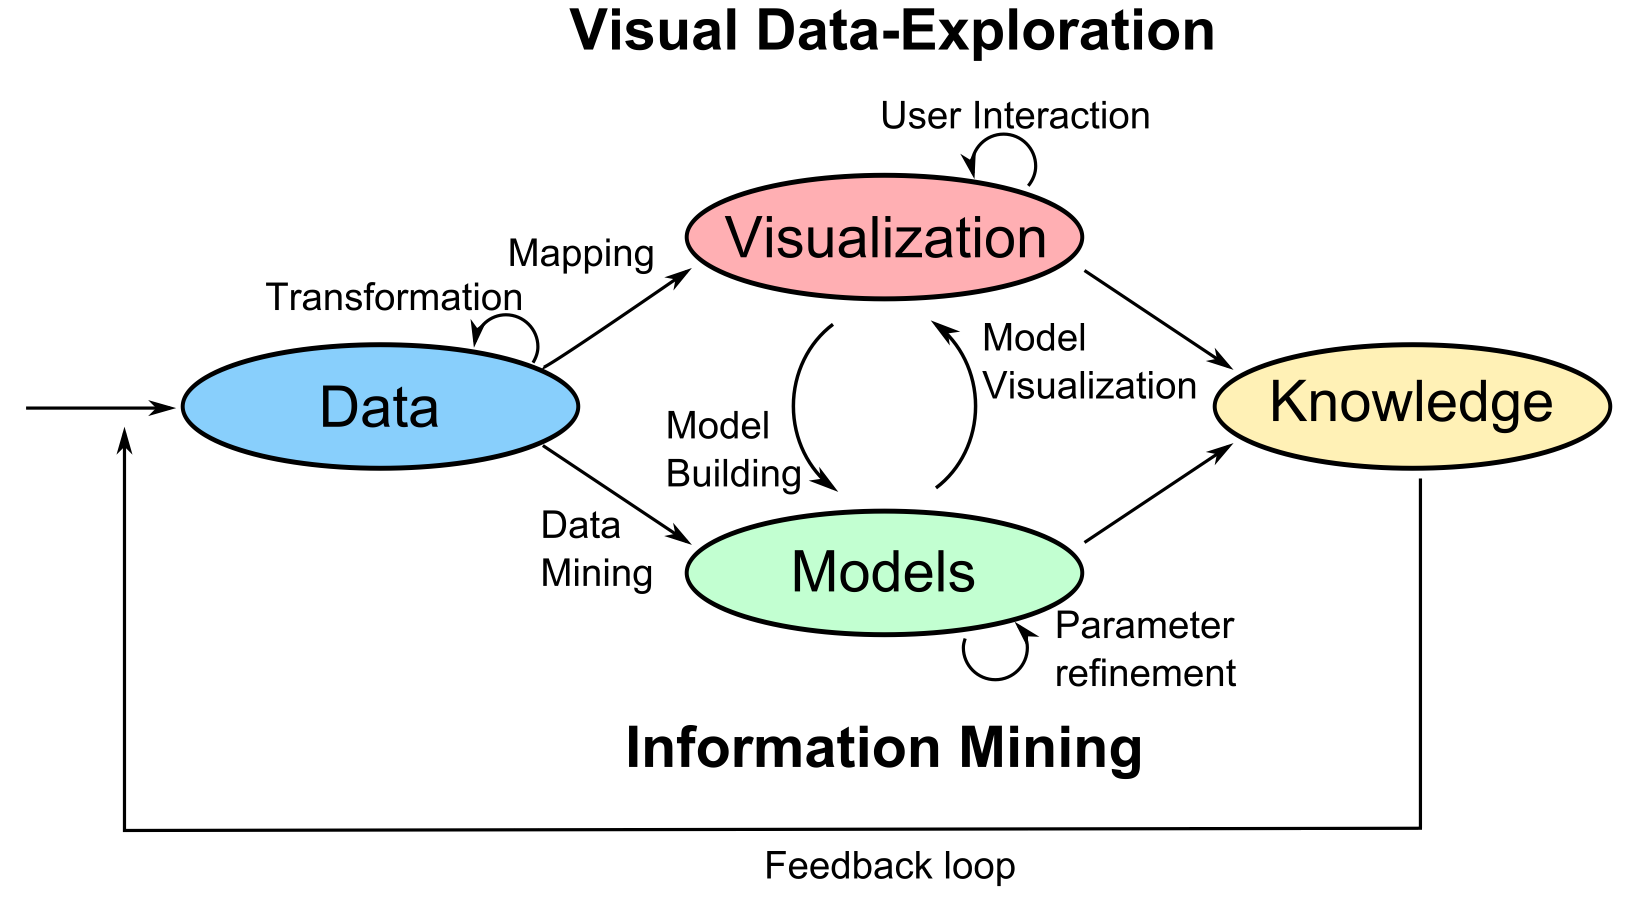
\includegraphics[width=.75\linewidth]{./figures/ch4/visual_analytics_process_keim}}
    \caption[Schéma du processus de \textit{Visual Analytics} proposé par Keim \textit{et al.}.]{{\it Schéma illustratif du processus de Visual Analytics tel que proposé par Keim \textit{et al.}. Les différentes étapes sont illustrées par des ovales, les transitions par des flèches.}}
  \label{Fig:visual_analytics_process_keim}
  \hspace{0.3cm}
\end{figure}

L'approche par Visual Analytics vise à combiner différentes modalités de visualisation afin de faciliter l'extraction de connaissances par l'expert. Ce processus, expliqué par Keim et al. \cite{keim2010mastering}, forme ainsi une boucle d'analyse fermée (voir Figure \ref{Fig:visual_analytics_process_keim}) susceptible de raccourcir considérablement le processus standard et plus séquentiel entre visualisation moléculaire et analyse en la biologie structurale, présentés dans la Figure \ref{Fig:schema_seq_bio_struct}. Une nouvelle représentation de ce processus intégrant la boucle de visualisation analytique peut être observée dans la Figure \ref{Fig:schema_seq_bio_optim}. %La représentation de Keim met en avant les principales dimension des approches par Visual Analytics : l'interactivité entre les données de même nature, leur différentes modalités de visualisations, la modèlisation des données, et . 

Les méthodes de Visual Analytics supposent l'intégration de données d'entrée hétérogènes. Ces étapes de \textit{transformation et d'intégration} des données hétérogènes passent par le nettoyage de ces données, leur normalisation, leur groupement et leur intégration dans un formalisme commun. Ces étapes sont cruciales, car elles conditionnent la construction de relations à présenter entre les différentes représentation visuelles scientifiques ou analytiques entre les données. %Certaines données et méthodes interactives de visualisation (détaillées dans la section \ref{visu_ana_tools}) permettent l'\textit{extraction de nouvelles connaissances} sans formatage particulier des données d'entrée. Cependant, dans la plupart des cas, la \textit{visualisation} seule n'est pas suffisante pour extraire de telles connaissances et elle doit être couplée à une étape d'\textit{analyse}. 

%Cette étape prend à la fois les données organisées par l'étape de \textit{transformation} mais également les données filtrées par l'étape de \textit{visualisation} afin d'appliquer des méthodes d'analyses automatiques ou semi-automatiques. Les résultats d'analyse peuvent constituer directement de nouvelles connaissances ou être eux-mêmes visualisés afin d'exploiter l'expertise de l'utilisateur pour extraire les nouvelles connaissances. Les étapes d'\textit{analyse} et de \textit{visualisation} impliquent toutes deux l'intervention de l'expert et implémentent donc une couche d'interaction permettant de guider les méthodes utilisées vers le cercle d'information que l'utilisateur considère comme important. Lorsque de nouvelles connaissances sont extraites, elles sont retournées comme données d'entrée dans la boucle de visualisation analytique et les étapes précédentes sont répétées.

La création de nouvelles connaissances passe par une exploitation plus efficaces des capacités cognitives de l'humain, supportées par des techniques de Visual Analytics à travers 6 moyens principaux :  \cite{card1999readings,cook_illuminating_2005} :

\begin{enumerate}
  \item en exploitant plus efficacement les ressources cognitives du sujet
  \item en réduisant le temps de recherche, grâce à la représentation de grandes quantités de données dans un petit espace par exemple
  \item en améliorant la reconnaissance de motifs, en organisant spatialement l'information de manière appropriée
  \item en soutenant l'inférence perceptive faciliter par la mise en relation des données, 
  \item par la surveillance perceptive d'un grand nombre d'événements potentiels, et
  \item en fournissant des représentations graphiques manipulables et dynamique, à la différence des graphes statiques, permettant une exploration interactive permettant de couvrir de manière interactive tout l'espace dans lequel sont défini les données analysées.
\end{enumerate}

Ces recommandations ergonomiques guident le développement de nouvelles générations d'applications dédiées à la visualisation analytique.

\begin{figure}
  \centering
  {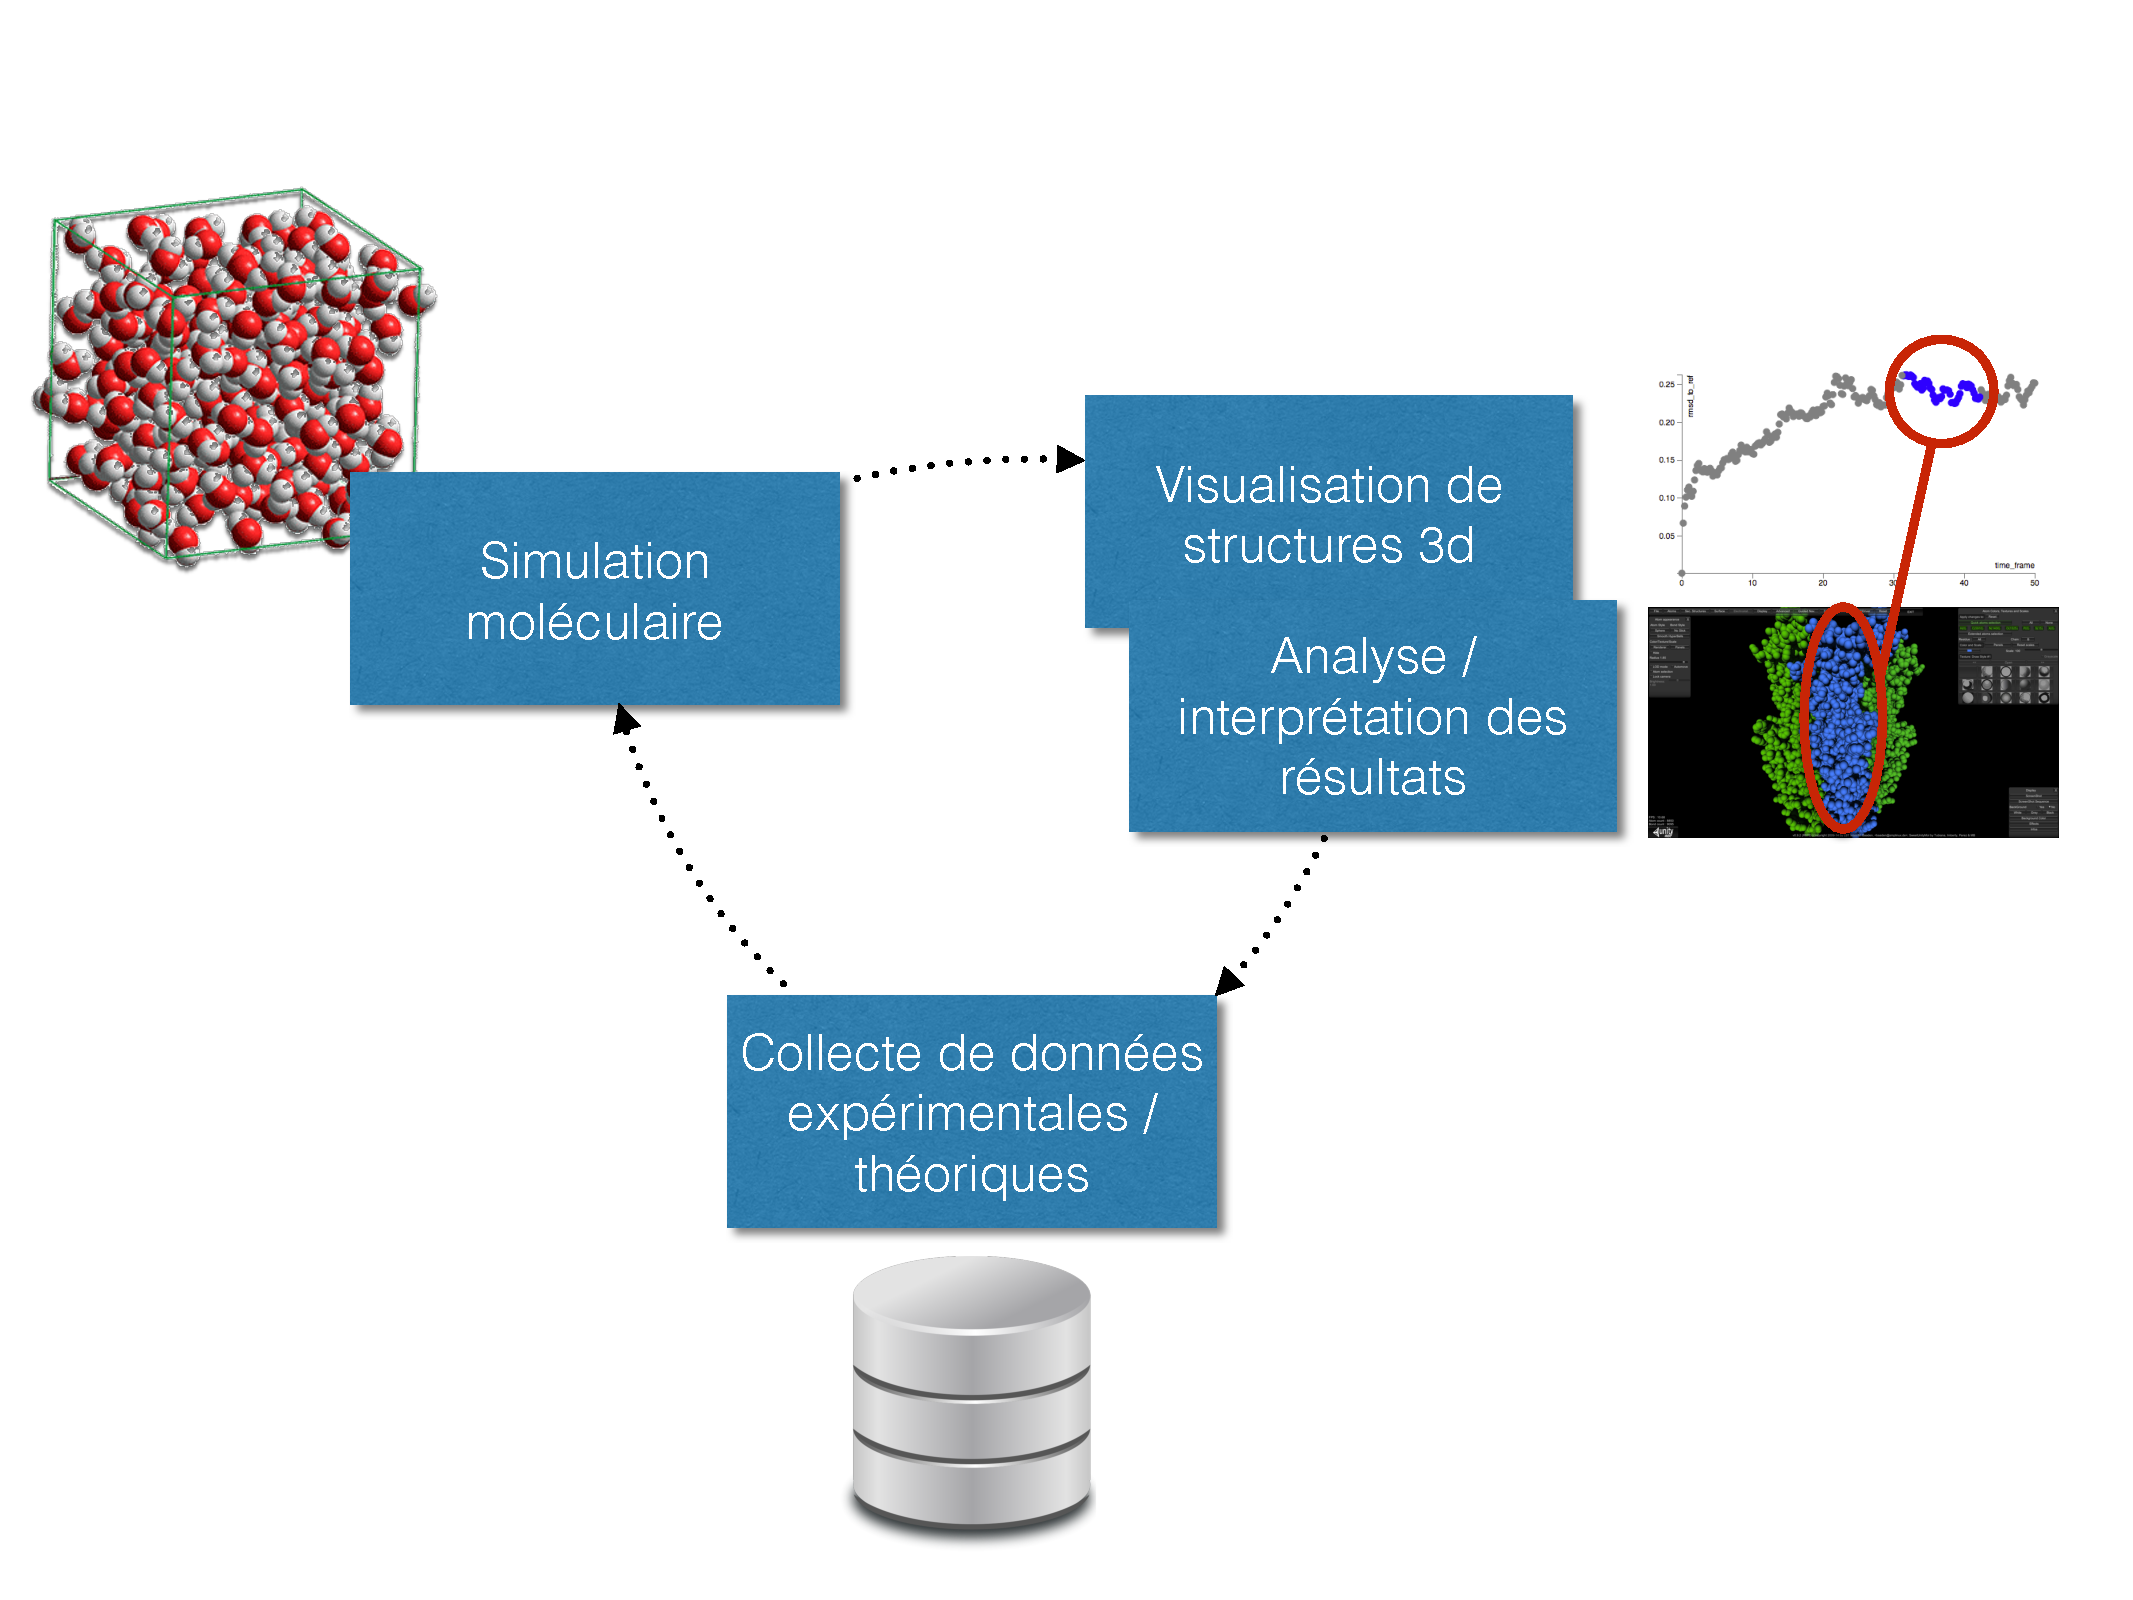
\includegraphics[width=.75\linewidth]{./figures/ch2/ch2_structural_biology_optim.pdf}}
    \caption[Processus séquentiel optimisé pour l'étude d'un système moléculaire en biologie structurale.]{{\it Processus séquentiel optimisé pour l'étude d'un système moléculaire en biologie structurale.}}
  \label{Fig:schema_seq_bio_optim}
  \hspace{0.3cm}
\end{figure}


\subsection{Outils et techniques} \label{visu_ana_tools}

Plusieurs outils ou techniques découlent de ce couplage étroit entre visualisation de données brutes et analyses associées en Visual Analytics.

\begin{enumerate}
    \item <<Overview+Detail>>: Cette technique met en relation plusieurs vues, synchrones ou asynchrones et dont l'une présente une vue globale du sujet,le tout dans des espaces visuels distincts. L'absence de synchronisation peut se retrouver dans la vue globale ou dans la vue détaillée. Une interaction dans l'une ou les autres des vues n'entraîne pas obligatoirement un changement dans les autres vues. Cependant, dans la plupart des cas, les vues sont synchrones et une cohérence est assurée entre les données affichées afin de pouvoir lier leur contenu. Une application connue de cette technique est retrouvée dans les programmes de visualisation de cartes comme illustrée dans la Figure \ref{Fig:overview+detail}. Ces visualiseurs de cartes géographiques présentent deux échelles spatiales différentes dans deux fenêtres distinctes. Seule l'interaction dans la fenêtre de contexte globale (la plus grande / principale) a un effet dans la seconde fenêtre.
    \item <<Zooming>>: Cette technique se base cette fois sur une séparation temporelle des vues. Un zoom avant amènera une vue plus détaillée d'une scène alors qu'un zoom arrière apportera une vue plus globale. La transition entre les différentes échelles de vue peut être continue ou discrète et présenter une animation ou non. L'un des problèmes majeurs de cette technique est la difficulté pour l'utilisateur d'inverser une action de zoom. En effet, la notion de défaire ou d'annuler une action en informatique fait souvent référence à des actions ayant eu pour effet de modifier l'état des données et non la vue de l'utilisateur.
    \item <<Focus+Context>>: Cette technique permet à l'utilisateur de se concentrer sur une partie intéressante des données visualisées sans perdre le contexte global dans lequel s'inscrivent ces données. Les informations présentées dans le contexte global ne sont pas nécessairement identiques à celles présentées en détail, mais les deux échelles d'information peuvent être associées à travers un affichage dynamique simple. Par exemple, si différents sets de données ont leurs entrées liées par au minimum une propriété équivalente, la sélection d'un point dans un set particulier sélectionne également tous les points correspondants à ce point dans les autres sets. La Figure \ref{Fig:focus+context} nous montre par exemple la sélection d'un ensemble de modèles dans un set de données de simulation moléculaire. Au moment de la sélection, toutes les représentations des modèles Y dans les espaces de visualisation ou d'analyse sont également sélectionnées et visuellement mises en avant. Cet exemple spécifique d'utilisation du focus+context est appelé \textit{brush-and-link} et se retrouve dans de nombreux logiciels de visualisation des données sous forme de graphiques simples.
    \item <<Cue-based techniques>>: Cette technique vise à mettre en avant un sous-ensemble de données intéressantes à l'utilisateur en intervenant sur la façon dont ces données sont affichées. A la différence des autres schémas décrits précédemment, elle n'intervient pas sur la taille des données, mais peut être utilisée en conjonction de chacune des techniques précédentes. Elle regroupe des méthodes de brouillage visuel des données, d'ajout de labels ou de mise en place d'éléments décoratifs divers pour attirer l'attention de l'utilisateur.
\end{enumerate}

\begin{figure}
  \centering
  {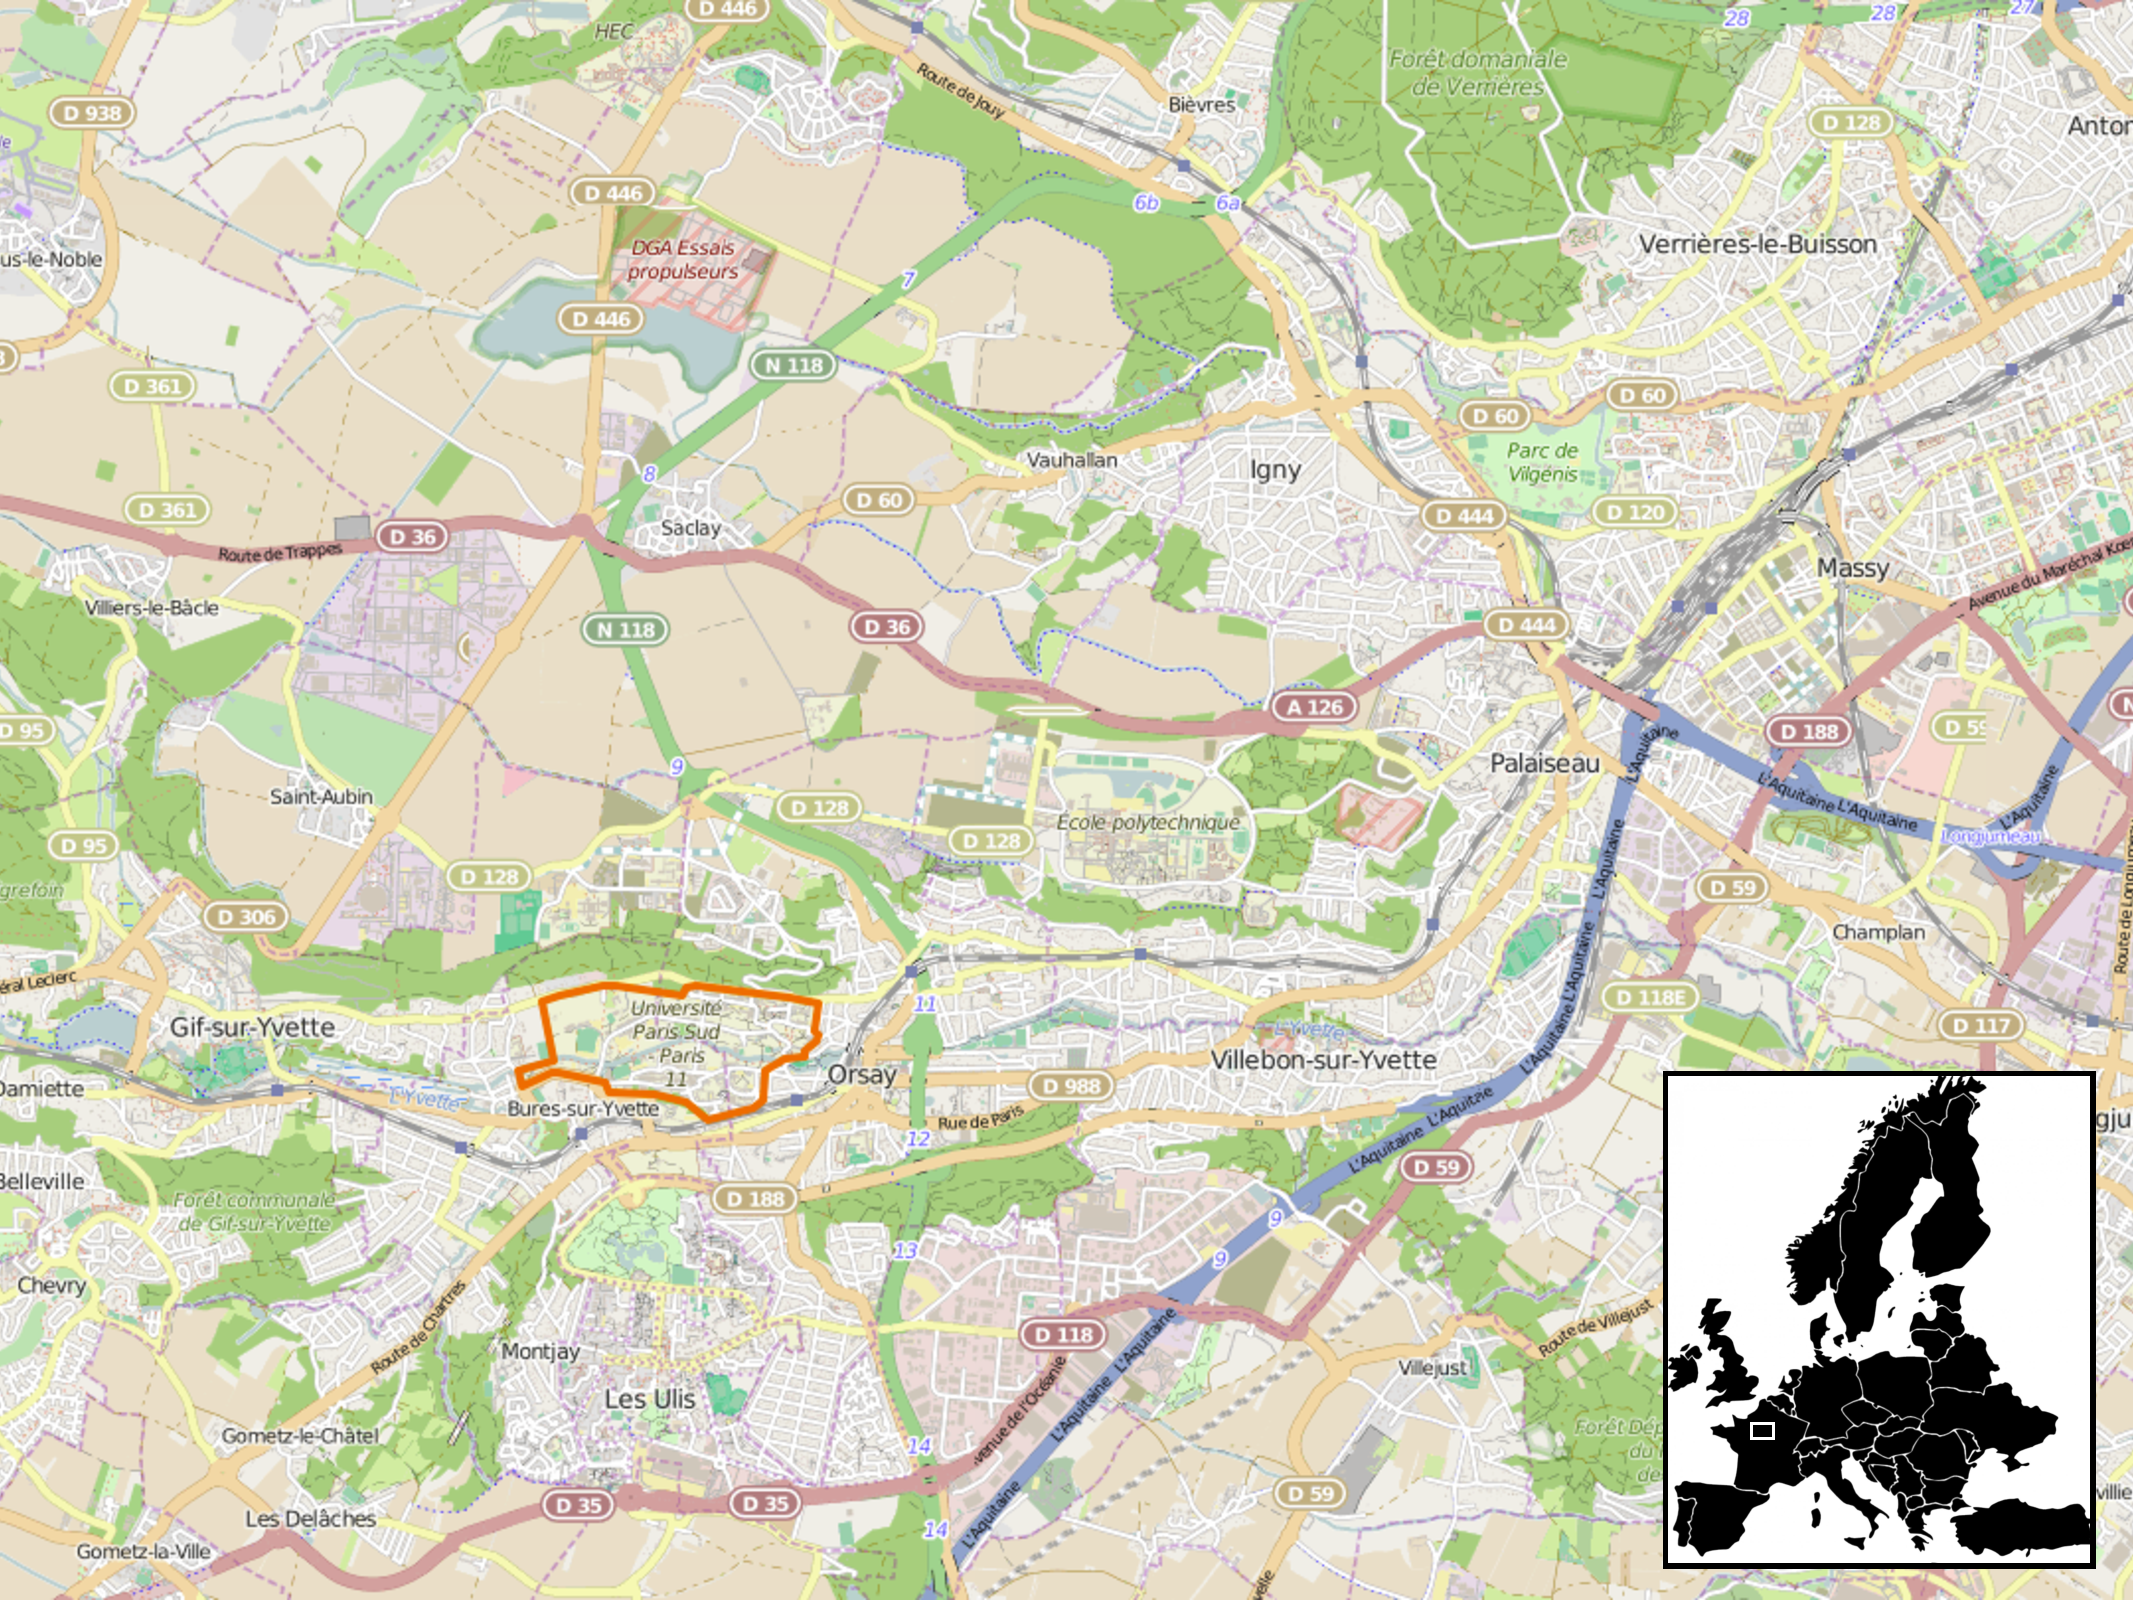
\includegraphics[width=.65\linewidth]{./figures/ch2/ch2_overview+detail}}
    \caption[Exemple utilisant la technique d'<<Overview+Detail>> sur une application de cartographie interactive.]{{\it Exemple d'application utilisant la technique d'<<Overview+Detail>> où un fond de carte principal possédant une certaine concentration d'informations et ciblant une région particulière (en couleur) est mis dans un contexte plus large et moins détaillé sur un deuxième fond de carte annexe (en noir et blanc).}}
  \label{Fig:overview+detail}
  \hspace{0.3cm}
\end{figure}

\begin{figure}
  \centering
  {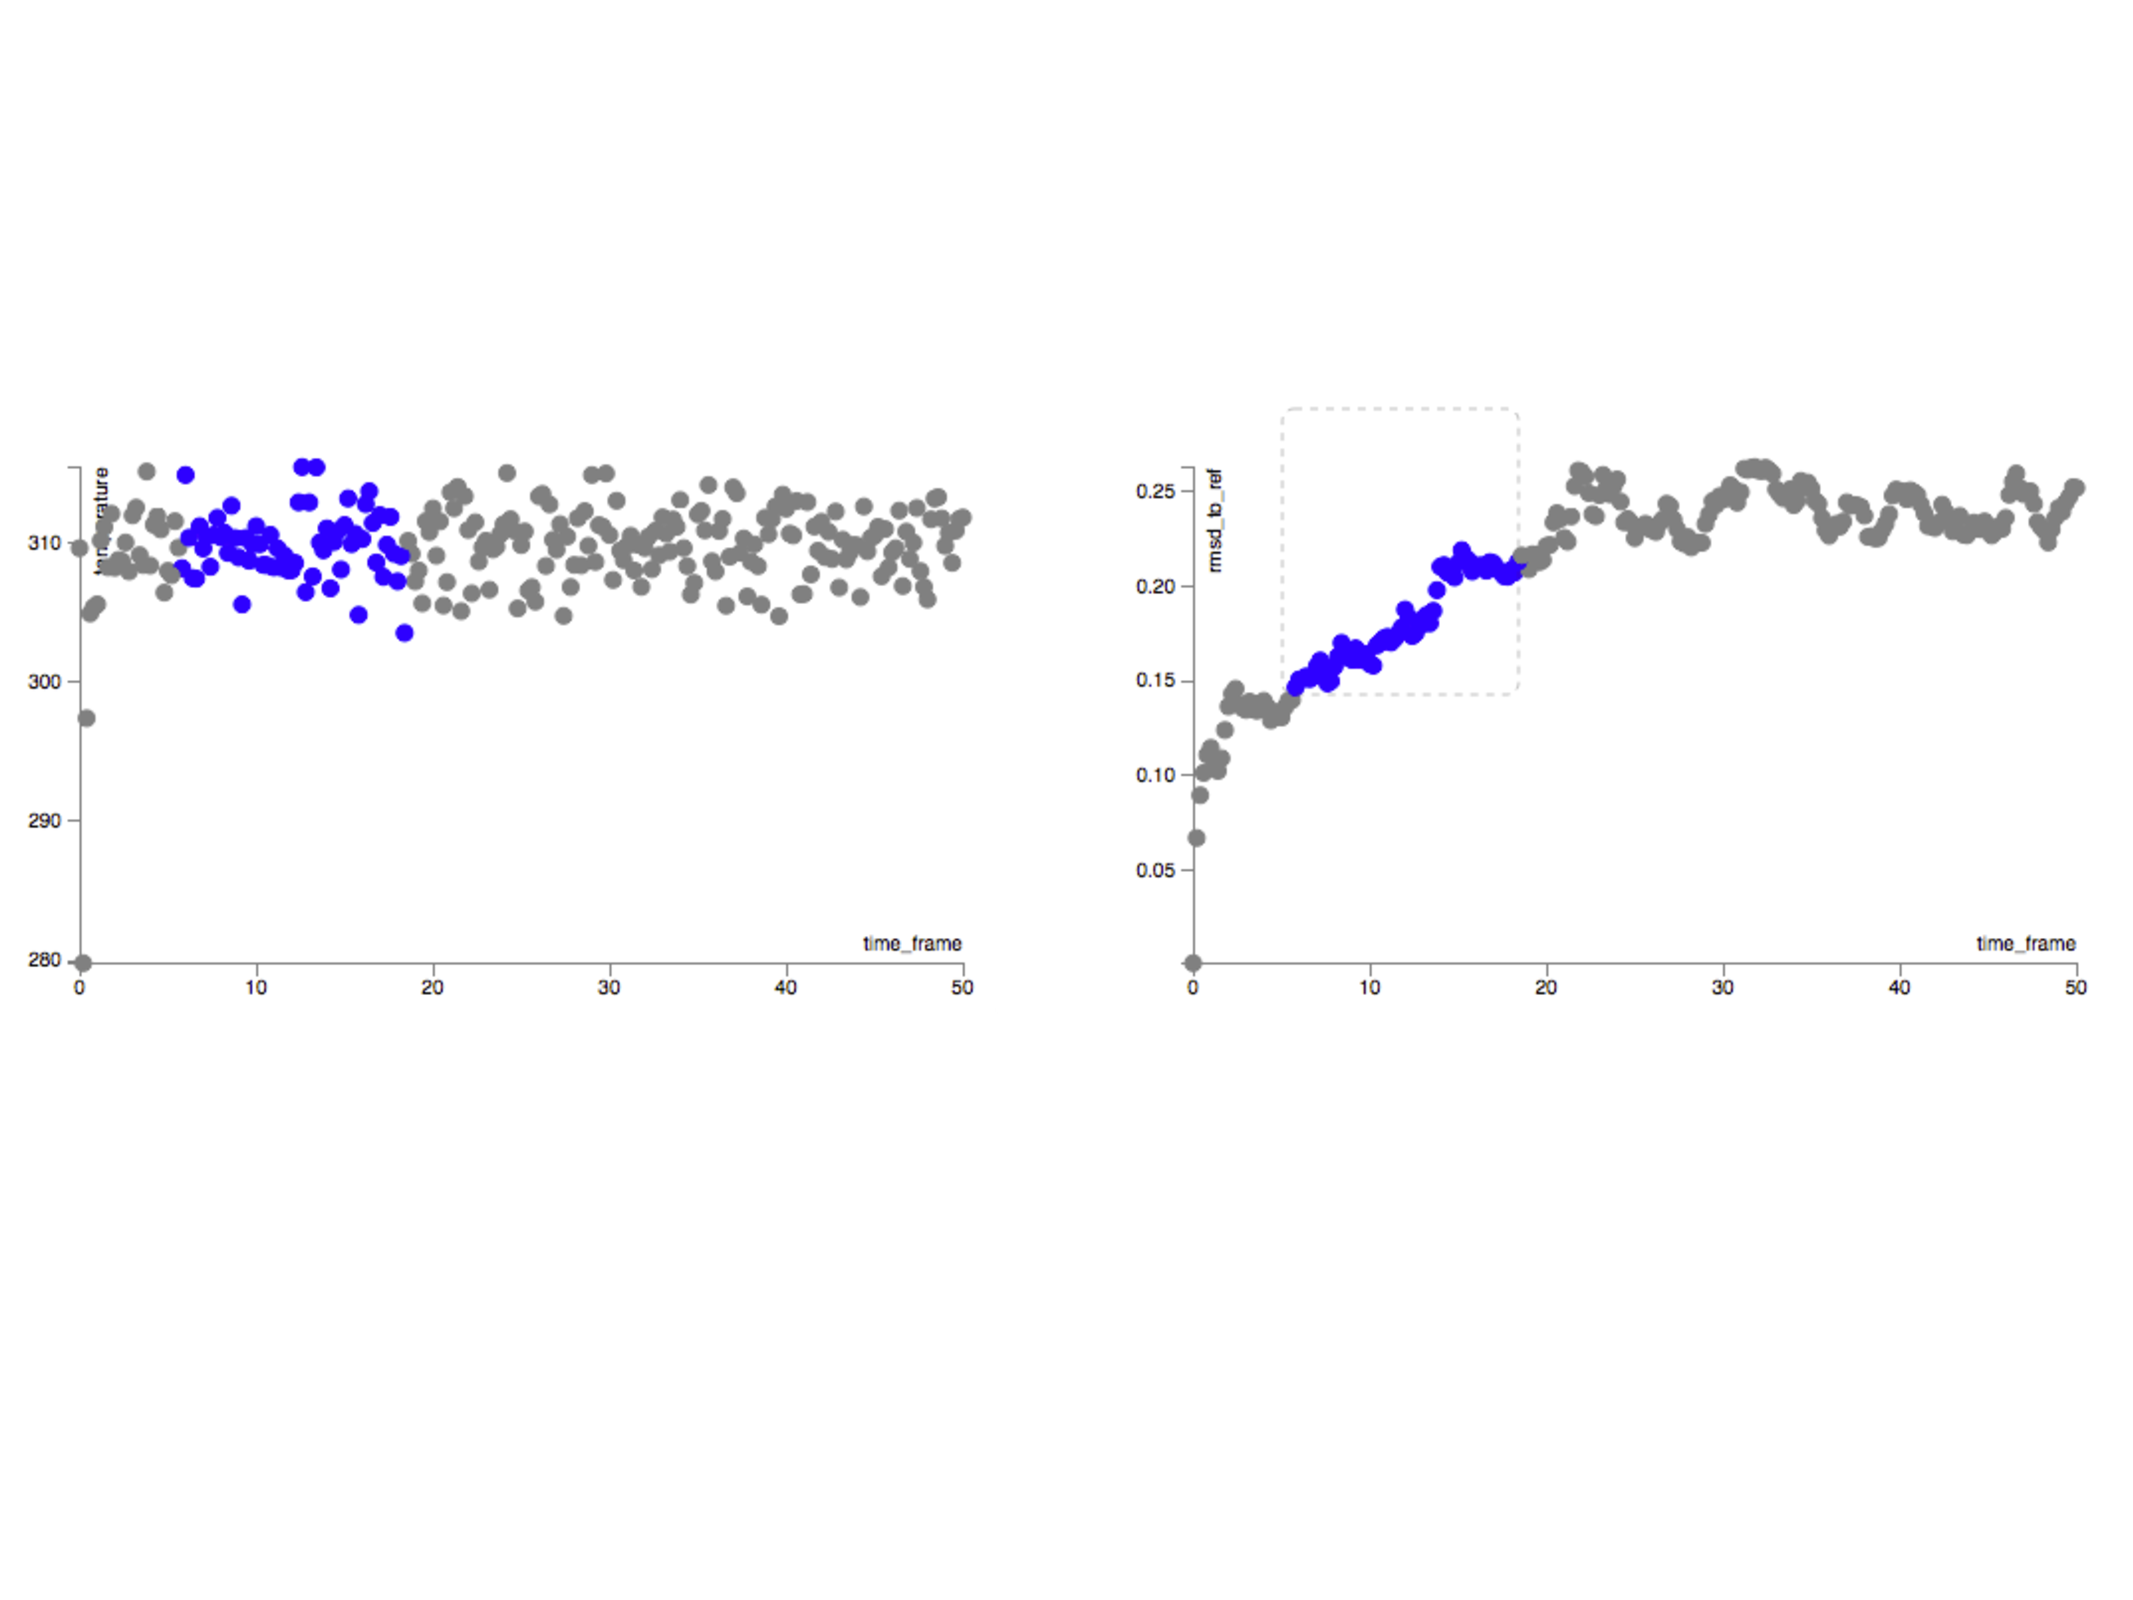
\includegraphics[width=.75\linewidth]{./figures/ch2/ch2_focus+context}}
    \caption[Illustration de la sélection simultanée et synchronisée d'un ensemble d'individus dans deux graphiques]{{\it Illustration de la sélection simultanée et synchronisée d'un ensemble d'individus dans les deux graphiques exposés. La sélection est effectuée dans le graphique de droite, mais se répercute dans le graphique de gauche.}}
  \label{Fig:focus+context}
  \hspace{0.3cm}
\end{figure}


\subsection{Applications en biologie structurale}
\label{Sec:visuAnalyticsStructBio}

Bien qu'étroitement associée à de nombreuses disciplines manipulant des jeux de données de grandes tailles, la visualisation analytique n'est que partiellement utilisée en biologie structurale. La dissociation actuelle entre analyses et visualisation peut expliquer ce retard dans son implémentation au sein des outils de visualisation et modélisation moléculaire.

La visualisation analytique possède pourtant les outils nécessaires au couplage visualisation et analyses propres à l'étude d'une simulation moléculaire. En reprenant le schéma de la visualisation analytique proposé par Keim \textit{et al.} \cite{keim2010mastering}, exposé dans la Figure \ref{Fig:visual_analytics_process_keim}, il est facile de considérer la sortie d'une simulation moléculaire (des coordonnées 3D de modèles + propriétés physico-chimiques) comme données d'entrée. En utilisant des rendus visuels définis pour chaque information à observer (rendu 3D navigable pour les coordonnées 3D des complexes moléculaires, plots et graphes pour les données d'analyses, etc.) et en liant ces rendus entre eux, il est possible de mettre en place des techniques de Focus+Context ou de Overview+Detail qui entraîneront l'adaptation synchronisée des espaces de visualisation et d'analyses \cite{schulz2011visual,kerren_toward_2012}.

On retrouve quelques caractéristiques de ce qu'apporte la visualisation analytique dans des applications comme KING \cite{chen_king_2009} ou DIVE \cite{rysavy_dive:_2014} cherchant à accroître la quantité d'informations disponibles pour l'utilisateur tout en maintenant un lien fort entre les données affichées. Une bonne présentation des informations dans leur contexte et la mise en place de connexions entre elles apportent un environnement de décision complet pour l'utilisateur. Cytoscape \cite{shannon_cytoscape:_2003,doncheva_topological_2012} est une plateforme logicielle permettant la visualisation de réseaux complexes, notamment biologiques, associée à de nombreux types de données tels des structures 3d protéiques, graphiques d'analyses, etc.

On retrouve parmi ces derniers exemples une volonté de mettre en relation certains jeux de données afin d'en extraire des corrélations de comportement permettant de soutenir ou d'infirmer des hypothèses déjà énoncées. Cette mise en relation est possible grâce au programme utilisé, cependant, le choix des données à afficher et éventuellement à lier est le fait de l'utilisateur. Ce dernier va se servir du programme dans le seul but de faire apparaître des données de façon organisée dans le but de mettre en place des liens logiques en vue d'extraire les connaissances supplémentaires. La démarche de notre étude va plus loin puisque nous allons chercher à anticiper les éventuelles connexions entre les données afin de fournir à l'utilisateur un environnement où la majeure partie de sa réflexion ne sera pas la mise en place cognitive de ces liens, mais plutôt la mise en place d'hypothèses scientifiques et l'acquisition de nouvelles connaissances. Le prérequis de cet environnement particulier repose sur la connaissance des données et comment les présenter de façon à ce qu'une simple observation de la part de l'utilisateur lui permette de dégager une information supplémentaire, absente du champ de valeurs brutes qu'il manipule.

\subsection{Homogénéité des données}

Différents mécanismes permettent d'apporter un degré d'homogénéité aux données afin de faciliter leur traitement. La mise en place de repères visuels (code couleurs ou formes géométriques par exemple) au sein des espaces de visualisation est un premier moyen. Lorsque les données physico-chimiques sont associées à des sous-ensembles de la protéine (hydrophobie des acides aminés, polarité des atomes, distance des atomes au centre de gravité de la protéine, etc.) alors un repère visuel est ajouté à la représentation 3d du sous-ensemble concerné. Les logiciels de visualisation moléculaire intègrent d'ailleurs souvent nativement ces standards de représentation même si leur paramétrisation n'est pas souvent directe et passe par un codage spécifique de l'information à afficher au sein par exemples des fichiers de coordonnées type PDB pris en entrée. Cette approche permet donc de mettre en relation des informations de manière extrêmement intuitive pour l'utilisateur accélérant ainsi son processus cognitif de fusion des informations mais ne peut prendre en compte l'ensemble des données, en particulier analytiques.

Il n'est pas possible de générer de tels liens entre des données provenant de sources tant hétérogènes sans devoir posséder un certain niveau d'organisation et de structuration des concepts qui seront utilisés. Cette structuration peut aisément passer par une étape préliminaire de représentation des connaissances venant poser une définition et des liens ou des propriétés entre les différentes notions manipulées afin de permettre d'y appliquer un raisonnement et une certaine automatisation du rapprochement des données et de leur association aussi bien visuelle qu'organisationnelle.


% Intro sémantique / données liées
\section{Représentation des connaissances}

Dans les sciences informatiques, la représentation des connaissances est souvent associée à la notion d'ontologie. Une ontologie se définit comme un ensemble structuré de concepts et de relations permettant de décrire tout ou une partie d'un domaine. Une image connue énonce que <<l'ontologie est aux données ce que la grammaire est au langage>>.

Intégrer une ontologie à un système d'information permet de déclarer formellement un certain nombre de connaissances utilisées pour caractériser les informations gérées par le système et de se baser sur ces caractérisations et la formalisation de leur signification pour automatiser des tâches de traitement de l'information.
Dans un moteur de recherche, cela se caractérise par exemple par la possibilité d’améliorer la recherche d'information dans sa précision, en évitant des ambiguïtés au niveau terminologique (provenant de l'homonymie) ou dans son taux de rappel, en intégrant des notions plus précises ou équivalentes (en utilisant la synonymie, l'hyponymie) ou en déduisant des connaissances implicites (par exemple, des règles d'inférence) ou en relâchant des contraintes trop strictes en cas d'échec de la requête (par généralisation) ou en regroupant des résultats trop nombreux selon leur similarité pour les présenter de façon plus conviviale (regroupement ou clustering conceptuel).

La notion de représentation des concepts et des liens entre ces concepts est connue des sciences informatiques et plusieurs formalismes en découlent. La mise en place d'ontologies afin de standardiser les connaissances dans des domaines de recherche scientifique a connu un développement spontané et important à partir de la fin des années 90 \cite{schulze-kremer_ontologies_2002, baker_ontology_1999}. 
Une ontologie est \textit{l'ensemble structuré des termes et concepts représentant le sens d'un champ d'informations, que ce soit par les métadonnées d'un espace de noms, ou les éléments d'un domaine de connaissances.}\footnote{\url{https://fr.wikipedia.org/wiki/Ontologie_\%28informatique\%29}}. Une ontologie se définit comme un vocabulaire cherchant à classer des concepts et définir des relations entre ces concepts pour un domaine spécifique. Ce classement hiérarchique se doit d'être interprétable à la fois par les machines et les humains. Tout d'abord afin d'être intégré dans des processus informatiques et ensuite afin de servir de modèle aux scientifiques pour l'élaboration de bases de données résultantes d'ontologies.


\subsection{Choix du formalisme}

Afin de correctement manipuler les connaissances et les données sous-jacentes, il convient de choisir un formalisme adapté à notre objectif. Le formalisme utilisé pour représenter des connaissances dépend à la fois du domaine d'application (ici la biologie structurale), des opérations à mettre en oeuvre sur ces connaissances (lier les faits entre eux, extraire de nouvelles connaissances, obtenir des descripteurs pertinents pour l'aide à la décision) et des processus d'implémentation qui seront utilisés (nous désirons utiliser ce formalisme au sein d'une suite logicielle multi composants performante). Au sein des formalismes, il est possible de distinguer deux classes d'approches, les approches non logiques et les approches logiques.

Les approches non logiques regroupent des logiques descriptives comme les \textit{réseaux sémantiques} et les \textit{Graphes Conceptuels} (GC).
Les approches logiques regroupent les \textit{logiques classiques} comme les logiques propositionnelles, de 1ers ordres ou de 2es ordres ainsi que les \textit{logiques de description}.

\subsubsection{Réseaux sémantiques}

Les réseaux sémantiques sont destinés à la modélisation hiérarchique de connaissances sous forme de graphes marqués. Un réseau sémantique contient des concepts, représenté par des noeuds et des relations, représentés par des liens (ou arcs) étiquetés entre chaque noeud. Ils ont été dans les années 60 par Quillian et Collins \cite{collins1969retrieval} comme base pour la représentation taxonomique. Ils se caractérisent par des relations binaires entre les concepts de type \textit{est-un}, \textit{a} ou \textit{type-de}.

\subsubsection{Graphes Conceptuels}

Les graphes conceptuels, introduits par Sowa en 1984 \cite{sowa1983conceptual}, tiennent leur origine des réseaux sémantiques \cite{lehmann1992semantic} et sont un moyen de formaliser les connaissances \cite{chein2008graph}. Ce modèle est mathématiquement fondé sur la logique et la théorie des graphes. Cependant, pour raisonner à l'aide de GC, deux approches peuvent être distinguées : (1) considérer les GC comme une interface graphique pour la logique et donc raisonner à l’aide de la logique et (2) considérer les GC comme un modèle de représentation à part entière disposant de ses propres mécanismes de raisonnement fondés sur la théorie des graphes. Dans ce modèle, les concepts et les relations sont des noeuds reliés par des arcs orientés comme illustrés dans la Figure \ref{Fig:conceptual_graph}. Les connaissances sont donc représentées par des graphes étiquetés dont les mécanismes de raisonnement se basent sur des opérations de graphes et en particulier sur l'\textit{homomorphisme} de graphes (anciennement \textit{projection}).
Un des inconvénients des GC réside dans leur faible utilisation au sein de la communauté scientifique. Peu de librairies ou applications supportant la notion de GC et la théorie des graphes qu'elle utilise existent. Leur implémentation au sein de suites logicielles en est donc partiellement difficile quand d'autres formalismes proches comportent une intégration plus importante au sein des langages de programmation les plus utilisés. De plus, ils sont exclusivement descriptifs et n'ont que peu d'extensions visées à leur adjoindre une sémantique basée sur la logique afin de pouvoir en extraire des connaissances supplémentaires.

\begin{figure}
  \centering
  {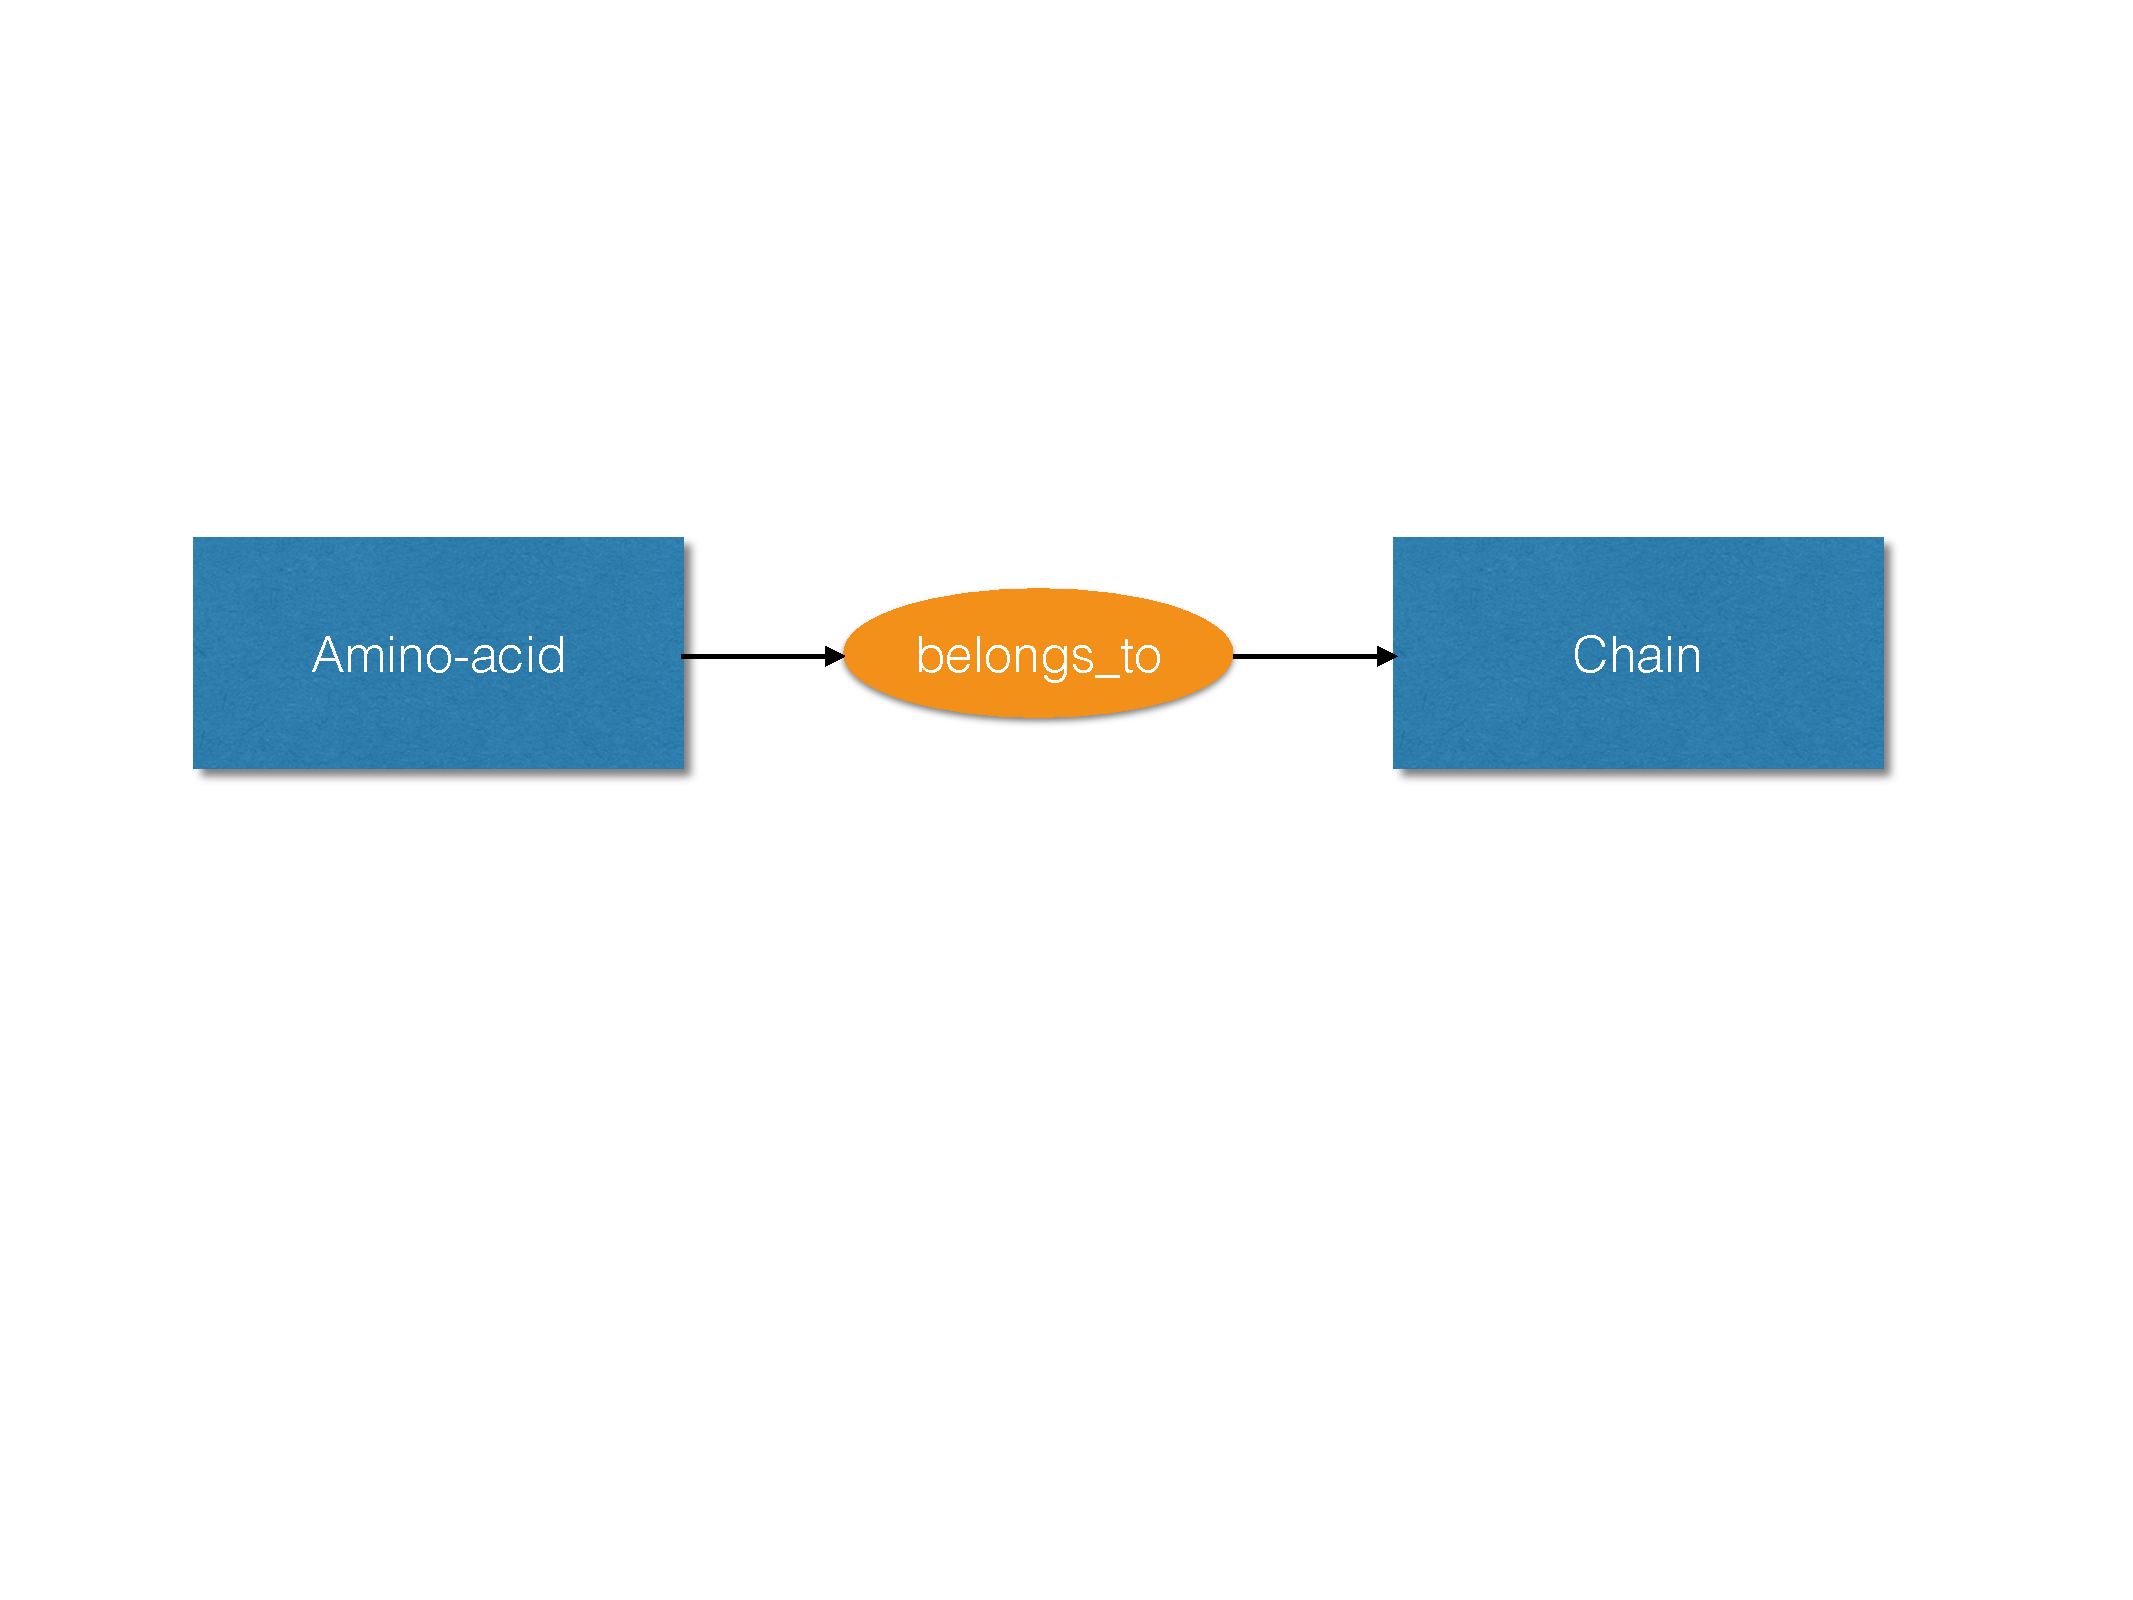
\includegraphics[width=.6\linewidth]{./figures/ch2/conceptual_graph}}
    \caption[Exemple de représentation sous forme de graphe conceptuel de deux concepts et une propriété en Graphe Conceptuel.]{\it Exemple de représentation sous forme de graphe conceptuel de deux concepts et une propriété. Ce sous-graphe est orienté (ici un acide aminé appartient à une chaîne, l'inverse n'est pas vrai) et étiqueté (les concepts sont $Amino-acid$ et $Chain$ et la propriété $belongs_to$).}
  \label{Fig:conceptual_graph}
  \hspace{0.5cm}
\end{figure}

\subsubsection{Logique classique}

Les logiques de 1er ordre, 2e ordre et propositionnelles sont 3 propositions de logiques dites <<classiques>> présentation une première formalisation du langage et du raisonnement mathématique. Cette logique est caractérisée par des postulats qui la fondent:

\begin{itemize}
  \item Le \textit{tiers exclu} énonce que pour toute proposition mathématique considérée, elle-même ou sa négation est vraie.
  \item Le \textit{raisonnement par l'absurde} qui veut prouver qu'une proposition est vraie non pas en la démontrant, mais on démontrant que la proposition contraire est absurde.
  \item La \textit{contraposition} qui consiste à dire qu'une implication de type <<A implique B>> permet de dire que <<si non-B alors non-A>>. B est donc une condition nécessaire de A.
  \item L'\textit{implication matérielle} ou le <<seulement si>> ou <<si ..., alors ...>> qui en logique classique se caractérise par la volonté de donner une valeur de vérité à toute proposition. Par exemple <<s'il pleut, alors mon gazon est mouillé.>> Cette proposition ne permet pas de dire, <<si mon gazon est mouillé, alors il pleut>>.
  \item Les \textit{lois de Morgan} qui sont des identités entre propositions logiques énonçant que <<non(A et B) est (non A) ou (non B)>> et <<non(A ou B) est (non A) et (non B)>>.
\end{itemize}

Parmi les logiques classiques, la logique du 1er ordre (ou calcul des prédicats) introduit les symboles mathématiques permettant de formuler des modèles de relations au sein d'ensembles mathématiques. On retrouve dans ces symboles: Les variables, les prédicats (ou relations), les connecteurs logiques (et, ou, etc.) et deux quantificateurs universel $\forall$ (<<Quel que soit>>, <<Pour tout>>) et existentiel $\exists$ (<<il existe au moins un ... tel que>>). Les formules logiques déduites des énoncés de calculs de prédicats ont pour but de s'appliquer à n'importe quel modèle où l'on retrouve des variables, des fonctions et des prédicats représentant respectivement les éléments de l'ensemble, les fonctions de l'ensemble et les parties (ou sous-ensembles) de l'ensemble.


\subsubsection{Logique de description}

Ces logiques se rapportent à la fois à la description des concepts décrivant un domaine et à la fois à la sémantique basée sur la logique. Cette logique est un apport par rapport aux réseaux sémantiques qui ne possèdent pas de sémantique basée sur la logique et sont donc exclusivement descriptifs. C'est une famille de langage permettant d'une part la description des connaissances d'un domaine de façon structurée et formelle et d'autre part elles possèdent une sémantique formelle définie en logique du 1er ordre. Elles sont utilisées pour de nombreuses applications, dont le web sémantique et la bio-informatique, au travers d'ontologies associées au domaine. 
Similairement aux logiques classiques, les logiques de description utilisent les notions de \textit{concept}, \textit{rôle} et \textit{individu} \cite{baader2003description}. Les \textit{concepts} désignent les sous-ensembles d'élément dans un univers étudié, les \textit{rôles} correspondent aux liens entre les éléments et enfin les \textit{individus} sont les éléments de l'univers.


\subsection{Logiques et ontologies en biologie}

La génomique fut le domaine biologique qui a vu le premier la nécessité d'utiliser des ontologies afin d'uniformiser la quantité de données toujours plus importante générée et intégrée dans des bases de données hétérogènes à travers le monde \cite{schuurman_ontologies_2008}.
En génomique et protéomique, de nombreuses études s'appuient sur l'aide directe ou indirecte de \textit{Gene Ontology} \cite{ashburner_gene_2000}, une <<bio-ontologie>> qui a résulté de la prolifération de jeux de données à l'échelle génomique et la mise en place de protocoles pour l'échange et le partage de données sur le web. Elle fut le fruit de la nécessité, lors de l'explosion du nombre de données générées, de mettre en place un vocabulaire standard que les scientifiques pourraient utiliser afin de classifier et renseigner leurs données. GO n'est pas totalement considéré comme une ontologie selon la définition informatique stricte du terme, car il ne possède pas de règles d'inférence complexes, ne se basant pas sur une description logique de ses concepts et sur des inférences simples de type \textit{est-un} ou \textit{est-une-partie-de}. Il est davantage mis en avant comme un vocabulaire standardisé des concepts mis en jeu dans les recherches afin de mettre en place un espace commun de termes précis et définis, possédant une hiérarchie établie. Il permet donc de mettre en relation des bases de données hétérogènes respectant ses codes ontologiques et donc d'effectuer des opérations de requêtes croisées ou de comparaison. Progressivement de nombreuses autres <<bio-ontologies>> sont apparues dans la lignée de GO et plusieurs d'entre elles ont permis de mettre en avant, au moyen du simple mécanisme d'inférence et de mise en relations des données hétérogènes, de nouvelles avancées en biologie \cite{yoshikawa_drug_2004, stenzhorn_biotop_2008, smith_obo_2007}.

Enfin, plusieurs programmes de visualisation analytique se sont appuyés sur la mise en place d'une sémantique décrivant les concepts mis en jeu \cite{rysavy_dive:_2014}. Cette représentation participe à la formalisation des concepts analysés et instaure un premier lien entre les différents modules d'un programme cherchant à partager visualisation et analyses au sein d'un même espace de travail. DIVE constitue un premier exemple de programme possédant un procédé logiciel incluant la mise en place automatique d'une ontologie afin de classer les données et de refléter le modèle de données utilisé par les librairies utilisées durant la session de visualisation et d'analyse. Le parseur mis en place dans DIVE traduit une architecture .NET \footnote{\url{https://microsoft.com/net}} en une structure de donnée hiérarchique. Chaque valeur de donnée est partagée entre l'architecture .NET et les représentations correspondantes dans DIVE permettant une modification/évolution dynamique de celle-ci pendant l’exécution du programme. Cette solution permet également de mettre en place des méthodes de requêtes sur les valeurs ou les relations entre les objets représentés et donc de mettre en avant de nouvelles informations sur les sets de données étudiés. DIVE se rapproche par plusieurs aspects de nos travaux, cependant, plusieurs points distinguent nos deux approches. Tout d'abord, afin de permettre un prétraitement et une harmonisation des données manipulées, notre ontologie est prédéfinie, imposant un contexte de travail précis et fixe. Cela favorise la mise en place de nouveaux modules, car l'utilisateur sait quels concepts et propriétés sont mis en jeu dans notre processus. Comme nous l'avons fait remarquer, notre ontologie garde une certaine souplesse puisqu'il est aisément possible de l'étendre à de nouveaux concepts et propriétés suivant les besoins. Il est cependant nécessaire de garder le vocabulaire de base de l'ontologie pour pouvoir profiter de toutes les fonctions en découlant. Notre ontologie est spécifique à notre domaine d'étude, qui est la biologie structurale et plus particulièrement la visualisation et l'analyse de données de modèles de molécules dynamiques ou non. DIVE est capable de fournir une architecture plus globale puisque s'adaptant à chaque set de données mis en jeu. L'inférence propre aux ontologies est également limitée dans DIVE puisqu'elle se limite à une notion d'héritage propre au modèle orienté objet de certains langages de programmation.

\subsection{Formalisme pour une représentation des données moléculaires en immersion}

Le formalisme employé au sein de notre application doit répondre à trois critères principaux:

\begin{enumerate}
  \item Représentation des données de façon hiérarchique au moyen de concepts et de propriétés.
  \item Possibilité de raisonner sur les données et d'extraire de nouvelles règles à partir des règles existantes
  \item Requêtes sur les données performantes pour introduire des mécanismes d'interaction respectant l'échelle de temps interactif
\end{enumerate}

Notre première implémentation d'une représentation des connaissances s'est faites au moyen de graphes conceptuels, formalisme familier de l'équipe, au sein de Cogitant. Les GC permettent de mettre en place une représentation hiérarchique des données et d’exécuter des requêtes de sélection, répondant ainsi à une partie de nos pré-requis. L'utilisation de représentations en GC souffre cependant de plusieurs limites de performances mis en lumière par Yannick Dennemont \cite{dennemont2013assistance} qui furent confirmés par nos retours d'utilisation.
La limitation des moyens de raisonnements ainsi que la faible utilisation au sein de la communauté nous a amené à considérer les logiques de description et le web sémantique comme base crédible de support pour la représentation de connaissances et l'extraction efficace d'informations au sein d'une base de faits. 

\section{Web sémantique et formalismes à base de graphes}


Le web sémantique est un mouvement collaboratif mené par le \textit{web Consortium} visant à développer des méthodes communes pour l'échange de données sur le web. Le but du web sémantique est de structurer et lier les connaissances présentes sur internet afin d'en faciliter le traitement et la recherche à travers le monde. Selon la définition même du W3C, \textit{le web sémantique fournit un modèle qui permet aux données d'être partagées et réutilisées entre plusieurs applications, entreprises et groupes d'utilisateurs.} Le concept de web sémantique n'est pas un modèle universellement adopté et, pour le moment, il se retrouve seulement dans plusieurs initiatives indépendantes attachées aux domaines de l'industrie, de la biologie et des sciences humaines. Historiquement, le web sémantique doit ses premiers pas à Tim Berners-Lee, le directeur actuel du W3C, qui pose les premières bases d'un environnement où les données seraient classées afin de pouvoir être rapidement mises en relation et partagées \cite{berners2001semantic}. Plusieurs chercheurs ont travaillé à son utilisation et les conséquences d'un passage de l'ensemble des acteurs du web à un tel concept \cite{feigenbaum_semantic_2007}. Nous pouvons citer comme initiatives notables DBpedia, un effort pour publier les données extraites de Wikipedia sous format RDF et interrogeables grâce à SPARQL que nous décrivons ci-après \cite{auer2007dbpedia} ou le projet Data.bnf.fr\footnote{\url{http://data.bnf.fr}} qui intègre des données provenant de formats divers (Itermarc\footnote{\url{http://www.bnf.fr/fr/professionnels/f_intermarc/s.format_intermarc_biblio.html}}, XML-EAD et Dublin Core \cite{weibel1998dublin} pour la bibliothèque numérique), les regroupant et les formalisant par des traitements automatiques et les publiant dans divers standards du web sémantique basé sur le RDF \textit{Resource Description Framework} (RDF-XML, RDF-N3 et RDF-NT, voir section \ref{rdf_model}).

Le web sémantique se base sur un formalisme grandement inspiré des logiques de description. A l'image de plusieurs modèles du web et de l'internet, le web sémantique est caractérisé par plusieurs couches de définition selon le schéma présenté dans la Figure \ref{web_semantic_tools}. Le modèle de graphe associé au web sémantique est le RDF \cite{klyne2006resource}. Il est structuré par le RDFS (RDF Schema) \cite{brickley2004rdf} qui décrit les vocabulaires (ontologies) sur lesquelles des ressources RDF se basent à la manière d'une DTD (Document Type Definition) pour le XML (eXtensible Markup Language) qui permet de mettre en place une hiérarchie au niveau des balises utilisées dans un document XML. 
L'ensemble des caractéristiques principales du RDFS est repris dans un langage ontologique plus expressif appelé OWL (Web Ontology Language)\cite{mcguinness2004owl}. OWL fonctionne de la même manière que RDFS en étendant certaines logiques sémantiques pour le RDF. La structuration des ressources RDF avec RDFS et OWL permet l'interrogation de ces ressources par le langage de requête SPARQL (SPARQL Protocol and RDF Query Language) \cite{prud2008sparql}. RDF, RDFS, OWL et SPARQL sont tous les 4 des recommandations du W3C pour le web sémantique et ils disposent d'une intégration de plus en plus élargie au sein des technologies et contenus web destinés au partage de connaissances et à leur traitement.

\begin{figure}
  \centering
  {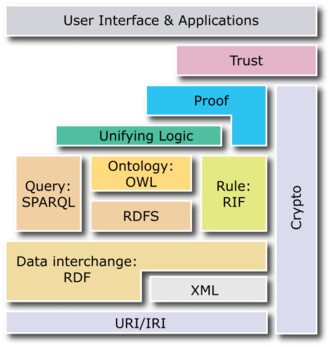
\includegraphics[width=.5\linewidth]{./figures/ch2/web_semantic_hierarchy}}
    \caption[Architecture du web sémantique et représentation de ses différentes couches.]{\it Architecture du web sémantique et représentation de ses différentes couches. Cette illustration reprend notamment les standards adoptés en web sémantique et utilisés pour chaque couche d'implémentation: RDF, RDFS, OWL, SPARQL, etc..}
  \label{Fig:web_semantic_hierarchy}
  \hspace{0.3cm}
\end{figure}

\subsection{Modèle RDF, formats et langages} \label{rdf_model}

Le langage RDF est le langage de base du web Sémantique qui l'utilise afin de mettre en place un réseau de données partagées et libres. C'est un modèle de graphe destiné à décrire de façon formelle des ressources et leurs métadonnées associées, de façon à permettre leur traitement automatique.

Le modèle RDF se base sur une représentation des connaissances à partir de triplets comme illustré dans la Figure \ref{Fig:rdf_hofstader} par Douglas R. Hofstader \cite{douglas1979godel}. Le triplet est la plus petite division de connaissances en RDF et toute description de données est un ensemble de triplets comprenant:

\begin{lstlisting}
(sujet, prédicat, objet)
\end{lstlisting}

\begin{figure}
  \centering
  {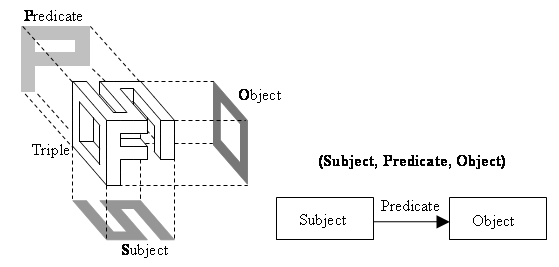
\includegraphics[width=.5\linewidth]{./figures/ch2/rdf_hofstader.png}}
    \caption{\it Illustration de la décomposition de base du langage RDF : sujet, prédicat, objet.}
  \label{Fig:rdf_hofstader}
  \hspace{0.3cm}
\end{figure}

Le \textit{sujet} représente la ressource que nous cherchons à décrire. Le \textit{prédicat} représente une propriété pouvant être associée à la ressource. L'\textit{objet} peut représenter soit une ressource, soit une donnée, cela correspond à la valeur de la propriété.
Chaque ressource est identifiée par un URI (Uniform Ressource Identifier) alors qu'une donnée est anonyme puisque pouvant être dupliquée (valeur numérique, chaîne de caractère, etc.). Un exemple de triplet pourrait être:

\begin{lstlisting}
http://mon-ontologie.fr/#Pierre   http://mon-ontologie.fr/#âge  xsd:int^^26
\end{lstlisting}

Les ressources de ce triplet (\textit{sujet} et \textit{prédicat}) sont décrites par leur URI qui est constitué d'une partie fixe (\textit{http://mon-ontologie.fr/\#}) identifiant le moyen de localiser la ressource et une partie variable (\textit{Pierre} et \textit{âge}) correspondant au nom de la ressource identifiée. Les URI les plus connues et utilisées sont les URL permettant d'accéder à des ressources internet, mais les numéros ISBN référençant les livres sont également des URI. La notion d'URI est importante dans le modèle RDF, car ce sont ces URI qui permettent de désigner de façon non ambiguë une ressource que l'on souhaite décrire. Lors de la mise en place d'une nouvelle base de données, il est courant de créer son propre domaine de définition ou préfixe afin d'identifier toute ressource, classe ou propriété nouvelle décrite. Dans la suite de ce chapitre, nous considérerons \textit{http://mon-ontologie.fr/\#} comme notre ensemble de définitions et nous le préfixerons grâce au mot-clé \textit{my}. En langage RDF, cela se caractériserait par la ligne suivante:

\begin{lstlisting}
@prefix my:    <http://mon-ontologie.fr/#>
\end{lstlisting}

La présence de cette ligne en en-tête d'un document RDF permet de réécrire l'exemple précédent:

\begin{lstlisting}
my:Pierre   my:âge  xsd:int^^26
\end{lstlisting}

Dans des termes propres aux bases de données relationnelles SQL, RDF peut être considéré comme une table composée de 3 colonnes, sujet, prédicat, objet. A la différence de SQL cependant, la colonne objet est hétérogène et le type de donnée par cellule est sous-entendue (ou spécifié dans l'ontologie, voir \ref{rdfs}) par la valeur du prédicat.

De la même manière que les graphes conceptuels, les documents RDF décrivant un ensemble de données peuvent être représentés par un multigraphe orienté étiqueté. Chaque triplet est représenté par un arc orienté dont les extrémités sont le sujet et l'objet et le label de l'arc correspond au prédicat. L'exemple précédent est illustré sous forme de graphe orienté ci-après:

\begin{lstlisting}
GRAPHE Pierre --âge--> 25
\end{lstlisting}

Fabien Gandon met très bien en avant le fait que le modèle RDF possède d'ailleurs plusieurs similarités avec le modèle des graphes conceptuels \cite{gandon_graphes_2008}. Ils partagent en effet la distinction entre sémantique (support pour les GC et schémas RDFS/OWL pour RDF) et la connaissance factuelle ou assertionnelle. Dans les deux modèles, cette connaissance est positive, conjonctive et existentielle, pouvant être représentée par des graphes orientés étiquetés. Les schémas RDF et GC possèdent une hiérarchie similaire des classes/propriétés pour RDF et concept/relation pour GC. Les relations et propriétés sont d'ailleurs indépendantes et définies en dehors des classes/concepts et se définissent donc comme de 1ers ordres dans la hiérarchie de ces deux modèles. Enfin, les deux modèles implémentent un mécanisme de déduction équivalent basé sur la subsomption en RDFS et la projection en GC. Ils s'éloignent cependant sur plusieurs points. Alors que RDF permet la multi-instanciation, GC ne possède pas d'équivalent. Une déclaration de propriété en RDF peut indiquer plusieurs domaines de définition et d'ensembles d'arrivée ce qui n'est pas le cas en GC. Les GC permettent par des relations d'arité supérieures à deux alors que les graphes RDF sont binaires. Les GC proposent également des extensions supérieures à l'expressivité de RDF/S.
Des travaux ont donc cherché à rapprocher ces deux formalismes afin de profiter de leurs avantages respectifs et gommer leurs défauts dans la mesure du possible. C'est le cas du projet CORESE \cite{corby_searching_2006} qui est un moteur de recherche s'appuyant sur le formalisme de RDF(S)/XML pour exprimer et partager ses données, mais utilise les mécanismes de requête et d'inférence fournis par les GC.

Les données RDF peuvent être représentées sous différents formats, du plus lisible pour l'être humain au plus optimisé pour le traitement informatique, souvent au détriment de sa lisibilité. De la même façon, ils peuvent répondre à différentes applications logicielles et donc ont été déclinés également pour leur intégration dans d'autres formats courants.

La syntaxe usuelle du RDF est le XML appelé \textbf{RDF/XML}. Le format par balises du XML et les attributs associés ainsi que sa possibilité de définir des hiérarchies sont des caractéristiques du RDF/XML particulièrement appréciés pour représenter des ressources et leurs propriétés. Cette syntaxe est définie par le W3C et fut le premier standard de format pour le modèle RDF \cite{beckett2004rdf}.

Le \textbf{RDFa} (RDF dans des Attributs) est un ensemble d'éléments et d'attributs permettant d'ajouter des données RDF à des documents HTML ou XML \cite{adida2008rdfa}. Il se base sur une partie de la syntaxe HTML qu'il reprend dans l'attribut \textit{classe}, qui va préciser le type de l'objet, l'attribut \textit{id}, qui va permettre de définir l'URI de l'objet et les attributs \textit{rel}, \textit{rev} et \textit{href} qui vont spécifier des relations avec d'autres ressources. Le RDFa possède également ses propres attributs dont les plus importants sont \textit{about}, permettant d'ajouter un URI décrivant la ressource décrite par les métadonnées, \textit{property} qui va permettre d'ajouter des propriétés à la ressource décrite.

Le \textbf{GRDDL} (pour Gleaning Resource Descriptions from Dialects of Languages) est un langage, recommandé par le W3C \cite{connolly2007gleaning}, permettant d'extraire des données RDF depuis un document XML ou XHTML grâce à des algorithmes de transformation et peut fonctionner comme implémentation du XSLT (Extensible Stylesheet Language Transformations, langage de transformation du XML en formats plus lisibles comme le HTML, le PDF ou le PNG par exemple).

La \textbf{Notation3} ou \textbf{N3} est une norme de sérialisation non XML pour le modèle RDF. Elle a été mise en place afin de fournir une syntaxe plus compacte et plus facile à lire. Elle a été développée, entre autres, par Tim Berners-Lee au sein de la communauté du web sémantique \cite{berners2008n3logic}. La norme N3 est davantage qu'une norme de sérialisation pour RDF puisqu'elle supporte également les règles basées sur RDF. Elle permet l'utilisation de symboles spécifiques pour éviter la répétition de motifs communs entre les triplets. Par exemple:

\begin{lstlisting}
my:Alanine  rdf:type  my:Acide-aminé ; 
  my:a-une-charge   my:Positive ; 
  my:est-composé-de   my:Carbon_alpha, my:Carbon_beta 
\end{lstlisting} 


Ici le <<;>> est utilisé afin de conservé le sujet (<Alanine>) alors que la <<,>> est utilisée pour conservé le sujet et le prédicat (<Alanine> et my:est-composé-de).

Le \textbf{Turtle} est un sous-ensemble de la syntaxe N3 n'existant pour le moment que sous forme de recommandation du W3C \cite{prud2013turtle}. Sa différence majeure avec le N3 est syntaxique. Il se rapproche beaucoup du format utilisé dans le langage de requête SPARQL (voir \ref{sparql}).

\textbf{N-Triplet} est un autre sous-ensemble de N3 beaucoup plus explicite puisque ne comportant pas de symboles particuliers simplifiant les descriptions de ressources. Son utilisation se limite souvent aux jeux de données RDF restreints, car son traitement a un coût computationnel assez élevé et la taille des fichiers générés est conséquente.

\textbf{JSON-LD} (ou JavaScriptObjectNotation for Linked Data) est une méthode de transmission des données liées RDF basée sur JSON. Pour rappel, JSON est un format standard ouvert largement utilisé dans les protocoles de communication asynchrones entre serveurs et clients web. Il se base sur la déclaration de structures clé/valeur, particulièrement adaptées à la description de concepts. 
Dans le cadre de JSON-LD, les clés sont les propriétés du concept, associées à leur valeur. Les valeurs peuvent être des références à d’autres concepts, des nombres ou encore du texte simple\footnote{\url{http://www.woptimo.com/2015/02/json-ld-la-revolution-semantique-des-microdonnees/}}. Deux propriétés sont obligatoires, \textit{context} et \textit{type}, et définissent respectivement l'ontologie utilisée et le meta-concept du concept courant (la ressource décrite). Un exemple de document JSON-LD est présenté ci-dessous:

\begin{lstlisting}[language=XML]
<script type="application/ld+json">
{
  "@context": "http://schema.org/",
  "@type": "Movie",
  "name": "Brannigan",
  "genre": "Thriller",
  "trailer": "https://www.youtube.com/watch?v=gAhzli9jbKU",
  "actors":
    {
    "@type": "Person",
    "name": "John Wayne",
    "birthDate": "1907-05-26"
    }
}
</script>
\end{lstlisting}

JSON-LD tend à devenir la nouvelle norme, majoritairement grâce à son interaction avec les bases de données, en particulier NoSQL. Le domaine du \textit{Big Data} connaît un essor exponentiel et beaucoup de grands acteurs du web (Google, Amazon, Twitter, etc.) migrent vers des paradigmes NoSQL, plus rapides. Les API qu'ils mettent à disposition sont accessibles à travers le protocole HTTP et utilisent le format JSON pour communiquer. Trois raisons principales pour l'utilisation de ce format: Sa compréhension aisée, sa structuration et son faible poids. L'ajout d'une couche sémantique avec JSON-LD en est donc grandement facilité. 

Nous avons vu que le modèle de représentation RDF s'appuie sur un formalisme précis et standardisé qui permet l'uniformisation des données représentées et la mise en place de lien entre ces données. Ce formalisme n'est qu'une méthode de représentation et ne constitue pas une logique de raisonnement qui permettrait d'extraire des connaissances de ces données. C'est dans ce but qu'ont été créés RDFS et OWL, des langages formels servant à décrire des ontologies. A la différence des données RDF qui sont de l'ordre du \textit{factuel}, une ontologie permet de décrire les concepts et les relations entre ces concepts et constitue la partie \textit{structurelle} du web sémantique.
OWL et RDFS reprennent les critères standards des ontologies existantes et qui sont le support de nombreuses ontologies recensées dans le portail officiel de bio-ontologies largement utilisées dans la communauté scientifique \cite{smith_obo_2007}.

\subsection{RDF Schema} \label{rdfs}

RDFS fut la première extension permettant d'ajouter une couche sémantique au modèle de ressource RDF. Il définit les notions de classes, sous-classes, propriétés et sous-propriétés desquelles dépendront les ressources RDF identifiées. C'est donc un ensemble de concepts haut-niveau définissant les différents individus d'un domaine et permettant leur hiérarchisation. 
Par exemple, RDF permet de décrire qu'une <Lysine> \textit{a une charge} <positive> grâce aux individus <Lysine> et <positive>, respectivement sujet et objet, et au prédicat \textit{a une charge}. RDFS permet d'ajouter les concepts décrivant les individus comme <Acide-aminé>, <Charge>, <Hydrophobicité>, <Molécule>, etc. et de préciser des relations entre ces groupes de façon à pouvoir émettre des déductions simples. Par extension de l'exemple précédent, si l'on ajoute que tout <Acide-Aminé> est une <Molécule> qui revient à dire en RDFS, <Acide-aminé> \textit{sous-classe de} <Molécule>, et <Lysine> \textit{instance de} <Acide-aminé>. Cela nous permet d'ajouter un niveau d'information induite des deux affirmations précédentes qui serait: <Lysine> \textit{instance de} <Molécule>. Cette déduction se fait grâce au système d'implication introduit par RDFS et permettant de déduire des informations complémentaires à partir d'un minimum de données.

RDFS introduit également la notion de domaine de définition (\textit{rdfs:domain}) et d'ensemble d'arrivée (\textit{rdfs:range}) pour les propriétés. Le domaine de définition correspond à la classe des sujets liés à une propriété alors que l'ensemble d'arrivée correspond à la classe ou au type de données des valeurs de la propriété. Il est par exemple possible de préciser que la propriété <identifiant> doit avoir comme domaine de définition seulement des individus de classe <Objets> et comme ensemble de définition des valeurs de type <xsd:integer>.
Le système d'implication de RDFS fonctionne également avec les notions de domaine d'application et d'ensemble de définitions. De ce fait, ces 3 affirmations:

\begin{lstlisting}
<my:Alanine>  <my:est-un>   <my:Acide-aminé> .
<myProtéine>  <my:contient> <my:Lysine> .
<my:contient> <rdfs:range>  <my:Acide-aminé> 
\end{lstlisting}

permettent d'induire l'affirmation suivante:

\begin{lstlisting}
<my:Lysine>   <my:est-un>   <my:Acide-aminé>
\end{lstlisting}

\subsection{OWL} \label{owl}

OWL est donc un standard informatique visant également à jouer le rôle de grammaire pour le langage RDF en complément du RDFS à qui il reprend ses bases. Le langage OWL se base sur des éléments des logiques de description et constitue un standard informatique permettant de vérifier que les données sont cohérentes, de déduire de nouvelles connaissances de ces données ou d'en extraire certaines informations.
Plus expressif que RDFS, OWL permet d'adjoindre à la définition des relations entre objets par des assertions fournies par RDFS, des propriétés reliant les classes à travers des relations de symétrie, d'équivalences, de cardinalité, etc. entre les classes. 
Il est donc possible de mettre en place des associations de classes et de propriétés plus complexes et basées sur une fondation logique  

Si l'on étend l'exemple précédent avec les notions apportées par OWL au sein des triplets suivants:

\begin{lstlisting}
<est-composé-de> \textit{est} <owl:TransitiveProperty>,
<Protéine> <est-composé-de> <Acide-aminé>,
<Acide-aminé> <est-composé-de> <Atome>
\end{lstlisting}

nous pouvons donc en déduire, grâce au caractère transitif de la propriété <est-composé-de>, que:

\begin{lstlisting}
<Protéine> <est-composé-de> <Atome>
\end{lstlisting}

De la même manière, il est possible de définir des propriétés comme symétriques, asymétriques, inverses, réflexives, etc.\footnote{\url{http://www.w3.org/2007/OWL/wiki/Quick_Reference_Guide}}
OWL est composé de 3 sous-langages classés du moins expressif au plus expressif: OWL-Lite, OWL-DL et OWL-Full. Parmi ces sous-langages, seul OWL-Lite est implémenté sous forme d'algorithmes décidables dans la majorité des moteurs d'inférence utilisés lors de l'interrogation de bases de données RDF possédant une ontologie OWL associée. La simplicité d'OWL-Lite lui permet une complexité réduite et donc un temps de calcul également réduit lors de son utilisation. Il regroupe les principales relations et descriptions de classe amenée par OWL et permet ainsi une mise en place de logiques descriptives suffisamment évoluées pour permettre l'extraction de nouvelles connaissances à partir de données simples.

\subsection{SPARQL} \label{sparql}

Nous venons d'évoquer la possibilité d'utiliser un moteur d'inférence afin d'extraire des données d'une base de données RDF. Cette extraction peut se faire grâce à l'utilisation d'un protocole et langage de requête appelé SPARQL. Ce langage permet à la fois de récupérer des données stockées sous format RDF dans une base de données, mais également de les éditer, d'en ajouter ou bien d'en supprimer. L'accès aux bases de données se fait grâce à une interface d'accès (en anglais \textit{endpoint}) géré par un service capable de recevoir des requêtes SPARQL et de renvoyer des résultats sous différents formats.
A la différence du SQL, SPARQL se base essentiellement sur le format en triplets des bases de données RDF et la majorité de ses requêtes repose sur la mise en place d'un schéma de correspondance entre triplets sujet/prédicat/objet. Il n'y a pas de contraintes de typage pour la colonne objet qui est habituellement implicite ou définie par l'ontologie. Dans le même esprit, l'ontologie est directement intégrée dans les résultats de requêtes et le schéma de données n'a donc pas besoin d'être appliqué de façon séparée. SPARQL fournit également plusieurs opérations sur les résultats comme SORT, JOIN, DISTINCT, qui permettent un traitement direct des résultats afin de les classer ou filtrer suivant les besoins...\footnote{\url{http://www.cambridgesemantics.com/semantic-university/sparql-vs-sql-intro}} Certains mots-clés de SQL ont été conservés tels que SELECT, FROM, WHERE, etc.
Une requête SPARQL se retrouve sous la forme suivante:

\begin{lstlisting}[language=SPARQL]
SELECT ?x ?id
FROM <http://my\_database.com> 
WHERE {
  ?y my:est-composé-de ?x .
  ?y rdf:type my:Chain .
  ?y my:chain\_id "B" .
  ?x my:res\_id ?id
}
\end{lstlisting}

Dans son fonctionnement, SPARQL va effectuer deux opérations successives sur la base de données. Une première étape est la recherche des triplets correspondant au modèle de triplet énoncé dans la requête. C'est l'étape de restriction qui va retourner l'ensemble des lignes de la base de données construites sur ce motif et comportant les valeurs spécifiées quand elles le sont (ici \textit{my:a-une-charge}, \textit{my:positive} et \textit{my:res\_id}). Cette étape se rapporte donc à ce qui se trouve dans le <<WHERE>>. Lorsque les triplets sont identifiés, SPARQL va sélectionner uniquement les variables demandées au niveau du mot-clé <<SELECT>>, ici ?x et ?id. C'est l'étape de projection qui va venir sélectionner les colonnes que l'utilisateur a demandé parmi les lignes sélectionnées dans l'étape précédente. Le résultat de la requête SPARQL précédente sur le jeu de données fourni en Annexe A pourrait donc être:

\begin{center}
 \begin{tabular}{|c | c|} 
 \hline
 ?x & ?id \\ [0.5ex] 
 \hline
 RES\_11 & 1 \\ 
 RES\_12 & 2 \\
 RES\_13 & 3 \\
 RES\_14 & 4 \\
 RES\_15 & 5 \\
 \hline
\end{tabular}
\end{center}

Les résultats sont présentés par défaut sous forme de tableaux par souci de clarté, mais la plupart des services SPARQL permettent leur conversion automatique en un nombre important de formats comme le XML, le JSON, JavaScript, Turtle, etc.
De nombreuses librairies utilisent des points d'accès SPARQL afin d'y présenter des requêtes et d'en récupérer leurs résultats. Cette implémentation présente dans de nombreux langages de programmation assure une certaine généricité du travail d'interfaçage nécessaire dans une suite logicielle multi composante.

\subsection{Implémentations et outils} \label{web_semantic_tools}

Nous avons évoqué la présence de librairies ou plateformes implémentant les standards du web sémantique et permettant d'utiliser ce modèle de représentation de données pour des activités hétérogènes. Nous pouvons citer plusieurs d'entre eux, associés fortement au web sémantique et cherchant à se développer parallèlement au domaine afin de lui offrir un support aussi complet que possible. Parmi ceux-ci:

\begin{itemize}
  \item \textbf{Jena}\footnote{\url{https://jena.apache.org/index.html}} \cite{mcbride2002jena} est l’un des moteurs actuels les plus complets et propose une persistance en mémoire ou en base de données. C'est une structure logicielle Java gratuite et ouverte implémentant RDF, RDFS et OWL ainsi que les requêtes SPARQL et propose un moteur en chaînage avant (RETE), arrière (programmation logique) et hybride. Ce moteur est utilisé pour implanter la sémantique de RDFS et OWL et son modèle repose sur une structure prédéfinie de bases de données.
  \item \textbf{Protégé}\footnote{\url{http://protege.stanford.edu/}} \cite{noy2001creating} est un outil basé sur Java et utilisé pour construire et éditer des ontologies. Il supporte RDF et OWL de façon native et intègre différents outils comme un visualiseur de réseau ontologique sous forme de graphe orienté ou une interface de requête SPARQL. Il est capable d'utiliser certains moteurs de logique de description afin d'inférer une ontologie ou de la valider.
  \item \textbf{Corese}\footnote{\url{http://wimmics.inria.fr/corese}} \cite{corby_searching_2006} est un moteur de recherche basé sur l'ontologie et rapprochant les approches de graphes conceptuels et de RDFS afin de répondre à des requêtes faites sur des annotations RDF. Il étend ainsi les règles d'inférence RDFS en s'appuyant sur certaines opérations propres aux graphes conceptuels.
  \item \textbf{Triple} \cite{sintek2002triple} est un langage de requêtes basé sur la logique de Horn permettant d'interroger des données du web sémantique et principalement des données RDF. Il est capable de raisonner grâce à des moteurs d'inférence et intègre les primitives RDF comme les espaces de nommage, les ressources et la notion d'individu (à opposer à concept ontologique). Son principal atout réside dans sa capacité à interroger différents modèles de données grâce à différentes logiques de description.
  \item \textbf{Fact} et son successeur \textbf{Fact++} \cite{tsarkov2006fact++} est un moteur à base de logiques de descriptions permettant de générer des requêtes conjonctives qui vont identifier, classifier ou valider des données d'une base de connaissances à partir de son ontologie. Ce moteur est à même de comprendre les ontologies OWL et donc d'appliquer les règles d'inférences qui lui sont associées. Il est par exemple implémentable dans l'outil Protégé cité précédemment.
  \item \textbf{jOWL}\footnote{\url{http://jowl.ontologyonline.org/}} est une librairie jQuery permettant de naviguer et de visualiser des documents OWL-RDFS au sein d'un environnement JavaScript et donc pouvant être intégré au sein de pages web.
\end{itemize}

\section{Conclusion}

La description du domaine du \textit{Visual Analytics} a mis en avant la nécessité de lier les données afin de permettre leur manipulation au sein de techniques qu'elle introduit. Ces données sont cependant hétérogènes dans le cadre du processus d'étude de structures moléculaires puisqu'elles sont à la fois de nature géométrique et de nature analytique. Des informations 3d (distance au ligand, poches de liaisons, etc.) doivent donc être partagées avec des informations 2d (énergie potentielle, charge, etc.). Pour les regrouper au sein d'un même contexte interactif, il est nécessaire de mettre en place un formalisme commun permettant de représenter l'ensemble des connaissances métier.

Parmi les formalismes à notre disposition pour cette représentation, la logique de description présente l'approche la plus en adéquation avec nos prérequis. Elle introduit la notion d'ontologie, utilisée par différents domaines d'application, en particulier biologiques, pour mettre en place une description des données utilisées et permettre leur réutilisation, comparaison et enrichissement autour d'un vocabulaire précis et formalisé dans l'ontologie. Les logiques de description permettent également d'étendre les connaissances d'une base de connaissances \textit{via} des relations logiques définies dans l'ontologie sans que ces relations factuelles soient explicitement présentes dans la base de connaissances.

La construction d'ontologies est la première étape du processus de formalisation sémantique des connaissances. Le web sémantique est une initiative présente dans de plus en plus d'institutions du web, nous avons choisi d'utiliser ses outils et modèles comme base de développement pour la description d'une plateforme cherchant à rassembler au sein d'une même représentation haut-niveau des concepts hétérogènes comme ceux mis en jeu au sein de la visualisation et de l'analyse de simulations moléculaires. Notre plateforme devra s'appuyer sur une représentation complète du contenu, du contexte interactif et de la tâche afin de permettre la liaison des données et leur manipulation  conjointe.

%%%%%%%%%%%%%%%%%%%%% FIN INTRO FROM CHAP.2 %%%%%%%%%%%%%%%%%%%%%%%%%%%%%%%
